\documentclass[12pt, a4paper, oneside]{ctexart}

\title{\kaishu\fontsize{24pt}{24pt}\selectfont 《面向对象程序设计》课程设计进度报告}
\date{}

\usepackage{graphicx}
\usepackage{listings}
\usepackage{xcolor}
\usepackage{float} % 导言区添加
\lstset{
  breaklines=true,             % 代码过长时自动换行
  columns=flexible,            % 让空格和中文显示更自然,防止对齐错乱
  basicstyle=\ttfamily,        % 代码使用等宽字体
  keywordstyle=\color{blue},   % 关键字高亮为蓝色
  commentstyle=\color{gray},   % 注释高亮为灰色
  stringstyle=\color{red},     % 字符串高亮为红色
  showstringspaces=false,      % 不显示字符串中的空格符号
  numbers=left,                % 在左侧显示行号
  numberstyle=\tiny,           % 行号使用小号字体
}

\begin{document}

% 标题
\maketitle

% logo
\vspace{-6em}  % 减少与标题的间距
\centering

\includegraphics[width=0.3\textwidth]{images/湖南理工学院logo..png}

% 基本信息
\vspace{2em}
\begin{flushleft}
\songti\fontsize{18pt}{18pt}\selectfont 课程设计题目:超市商品管理系统设计

\vspace{1em}
\songti\fontsize{18pt}{18pt}\selectfont \hspace{2em}专业班级:软件 23 - 1BF

\vspace{1em}
\songti\fontsize{18pt}{18pt}\selectfont \hspace{4em}姓名:胡岩松

\vspace{1em}
\songti\fontsize{18pt}{18pt}\selectfont \hspace{4em}学号:14234803500

\vspace{1em}
\songti\fontsize{18pt}{18pt}\selectfont 设计时间:2025-06-09 \hspace{4em}批阅时间:

\vspace{1em}
\songti\fontsize{18pt}{18pt}\selectfont 指导教师:廖军 \hspace{8em} 成绩:

\vspace{1em}
\songti\fontsize{18pt}{18pt}\selectfont 自评等级:良
\end{flushleft}

\newpage % 新的一页

% 目录
\clearpage
\tableofcontents
\clearpage

\newpage % 新的一页

% 正文

\section{题目分析}

\begin{flushleft}
课程设计题目为“超市商品管理系统设计”。题目要求实现一个能够对超市商品进行分类管理的系统,主要包括食品、化妆品、日用品和饮料四大类。每种商品都需包含名称、价格、库存量、生产厂家、品牌等基本信息。系统需完成商品的销售、统计、信息管理等基本操作。
\end{flushleft}

\section{需求分析}

\begin{flushleft}
(1)销售功能:根据商品类别和名称进行销售,校验库存,完成购买操作。

(2)添加功能:添加新的商品信息。

(3)查询功能:可按类别、名称、厂家条件查询商品信息。

(4)修改功能:修改已有商品信息。

(5)删除功能:可删除指定商品信息。

(6)统计功能:对商品数量、价格、库存等信息进行统计和排序。

(7)商品信息存盘与读取:商品信息的文件存储与读取。
\end{flushleft}

\section{功能设计}

\begin{flushleft}
(1)将商品包装成类,包含商品名称、价格、库存量、生产厂家、品牌等属性,便于对商品进行分类管理。

(2)设计一个超市管理系统类,包含商品列表等属性,并实现添加、查询、修改、删除等方法,由他对用户的操作进行响应。

(3)实现一个用户交互界面,提供菜单选项供用户选择操作。

(4)使用文件操作实现商品信息的读取和存盘,便于数据的持久化。

(5)实现销售功能,用户可以选择商品进行购买,系统自动校验库存并更新库存信息。

(6)实现增删改查等基本功能,让用户管理商品信息。
\end{flushleft}

\section{代码实现}


\textbf{1. 商品类(Product)}
\begin{lstlisting}[language=Java, breaklines=true]
// 定义商品类
public class Good {
    String type;            // 类别
    String name;            // 名称
    int price;              // 价格
    int remain;             // 库存量
    String manufacturer;    // 生产厂家
    String brand;           // 品牌

    Good(String type, String name, int price, int remain, String manufacturer, String brand) {
        this.type = type;
        this.name = name;
        this.price = price;
        this.remain = remain;
        this.manufacturer = manufacturer;
        this.brand = brand;
    }
}
\end{lstlisting}

\textbf{2. 超市管理系统类(Supermarket)}
\begin{lstlisting}[language=Java, breaklines=true]
// 定义超市类
public class Supermarket {
    // 将所有商品按类别放到四个集合里作为超市的一个元素
    Map<String, Set<Good>> goods;

    public Supermarket() {
        goods = new java.util.HashMap<>();
    }

    /*  菜单功能
     * 用户输入参数,系统调用方法。
     * */
    public void Menu() throws IOException {
        Scanner sc = new Scanner(System.in);
        System.out.println("正在进入超市管理系统...");
        System.out.println("*");
        System.out.println("*");
        System.out.println("*");
        System.out.println("超市管理系统进入成功!");
        System.out.println("键入Enter键继续...");
        sc.nextLine();

        while (true){
            // 用户输入操作类型,系统执行对应操作
            System.out.println("系统菜单如下:");
            System.out.println("1)销售功能      2)添加功能      3)查询功能      4)修改功能");
            System.out.println("5)删除功能      6)统计功能      7)信息存盘      8)信息读取");
            System.out.println("q)退出系统");
            System.out.println("请输入要执行的操作:");
            String mode = sc.nextLine();

            // 判断何时结束循环,退出系统
            boolean work = true;

            switch (mode) {
                case "1":
                    this.Sale_good(sc);
                    break;
                case "2":
                    this.Add_good(sc);
                    break;
                case "3":
                    this.Find_good(sc);
                    break;
                case "4":
                    this.Modify_good(sc);
                    break;
                case "5":
                    this.Delete_good(sc);
                    break;
                case "6":
                    this.Collect_goods();
                    break;
                case "7":
                    this.Save_data();
                    break;
                case "8":
                    this.Load_data();
                    break;
                case "q":
                    work = false;
                    break;
                default:
                    System.out.println("输入非法!请重新输入!");
            }
            // 当用户按退出键时退出管理系统
            if (!work){
                System.out.println("正在退出超市管理系统...");
                System.out.println("*");
                System.out.println("*");
                System.out.println("*");
                System.out.println("超市管理系统退出成功!");
                break;
            }

            // 等待用户键入Enter键再继续下一次循环,为用户留出反应时间
            System.out.println("[请键入Enter键继续...]");
            sc.nextLine();
            System.out.println();
            System.out.println();
            System.out.println();
        }

        sc.close();
    }

    /*  销售功能
     * 购买商品时,先输入类别,然后输入商品名称,并在库存中查找该商品的相关信息。
     * 如果有库存量,输入购买的数量,进行相应计算。
     * 如果库存量不够,给出提示信息,结束购买。
     * */
    private void Sale_good(Scanner sc){
        // 按类别查找商品
        System.out.println("请输入您要购买的商品类别:");
        String type = sc.nextLine();
        Set<Good> good_set = goods.get(type);
        if (good_set == null) {
            System.out.println("该商品类别不存在!");
            return;
        }

        // 按名称查找商品
        System.out.println("请输入您要购买的商品名称:");
        String name = sc.nextLine();
        Good good = null;
        for(Good g : good_set){
            if(g.name.equals(name)){
                good = g;
                break;
            }
        }
        if (good == null) {
            System.out.println("该商品不存在!");
            return;
        }

        // 计算库余量
        System.out.println("请输入您要购买的商品数量:");
        int num = Integer.parseInt(sc.nextLine());
        if (num > good.remain){
            System.out.println("很抱歉,该商品库余量不足!");
            return;
        }
        // 更新库存量
        good.remain -= num;
        // 计算总价
        int price = num * good.price;
        System.out.println("您一共消费" + price + "元!感谢惠顾!");
    }

    /*  添加功能
     * 主要完成商品信息的添加。
     * */
    private void Add_good(Scanner sc){
        System.out.println("请输入商品类别:");
        String type = sc.nextLine();
        System.out.println("请输入商品名称:");
        String name = sc.nextLine();
        System.out.println("请输入商品价格:");
        int price = Integer.parseInt(sc.nextLine());
        System.out.println("请输入商品库存量:");
        int remain = Integer.parseInt(sc.nextLine());
        System.out.println("请输入生产厂家:");
        String manufacturer = sc.nextLine();
        System.out.println("请输入品牌:");
        String brand = sc.nextLine();

        Good good = new Good(type, name, price, remain, manufacturer, brand);
        goods.computeIfAbsent(type, k -> new java.util.HashSet<>()).add(good);

        System.out.println("商品添加成功!");
    }

    /*  查询功能
     * 可按商品类别、商品名称、生产厂家进行查询。
     * 若存在相应信息,输出所查询的信息;
     * 若不存在该记录,则提示“该记录不存在!”。
     * */
    // 方法变种1:用于用户查找物品
    private void Find_good(Scanner sc){
        System.out.println("请输入您要查询的商品类别:");
        String type = sc.nextLine();
        System.out.println("请输入您要查询的商品名称:");
        String name = sc.nextLine();
        System.out.println("请输入您要查询的生产厂家:");
        String manufacturer = sc.nextLine();

        // 判断是否存在查询的商品类别
        Set<Good> good_set = goods.get(type);
        if (good_set == null) {
            System.out.println("该记录不存在!");
            return;
        }
        // 判断是否存在查询的商品名称和生产厂家
        Good good = null;
        for (Good g : good_set) {
            if (g.name.equals(name) && g.manufacturer.equals(manufacturer)) {
                good = g;
                break;
            }
        }
        if (good == null) {
            System.out.println("该记录不存在!");
            return;
        }

        // 若查询到商品信息,则输出查询结果
        System.out.println("查询结果:");
        System.out.println("[类别:" + good.type + "]");
        System.out.println("[名称:" + good.name + "]");
        System.out.println("[价格:" + good.price + "]");
        System.out.println("[库存量:" + good.remain + "]");
        System.out.println("[生产厂家:" + good.manufacturer + "]");
        System.out.println("[品牌:" + good.brand + "]");
    }
    // 方法变种2:用于其他函数调用
    private Good Find_good(String type, String name) {

        // 判断是否存在查询的商品类别
        Set<Good> good_set = goods.get(type);
        if (good_set == null) {
            return null;
        }
        // 判断是否存在查询的商品名称和生产厂家
        Good good = null;
        for (Good g : good_set) {
            if (g.name.equals(name)) {
                good = g;
                break;
            }
        }
        return good;
    }

    /*  修改功能
     * 根据查询结果对相应的记录进行修改。
     * */
    private void Modify_good(Scanner sc) {
        System.out.println("请输入您要修改的商品类别:");
        String type0 = sc.nextLine();
        System.out.println("请输入您要修改的商品名称:");
        String name0 = sc.nextLine();
        Good good = Find_good(type0, name0);
        if (good == null) {
            System.out.println("没有查询到商品信息,修改失败!");
            return;
        }

        System.out.println("请更新商品类别(当前:" + good.type + "):");
        String type = sc.nextLine();
        System.out.println("请更新商品名称(当前:" + good.name + "):");
        String name = sc.nextLine();
        System.out.println("请更新商品价格(当前:" + good.price + "):");
        int price = Integer.parseInt(sc.nextLine());
        System.out.println("请更新商品库存量(当前:" + good.remain + "):");
        int remain = Integer.parseInt(sc.nextLine());
        System.out.println("请更新生产厂家(当前:" + good.manufacturer + "):");
        String manufacturer = sc.nextLine();
        System.out.println("请更新品牌(当前:" + good.brand + "):");
        String brand = sc.nextLine();

        // 更新商品信息
        good.type = type;
        good.name = name;
        good.price = price;
        good.remain = remain;
        good.manufacturer = manufacturer;
        good.brand = brand;

        System.out.println("商品信息修改成功!");
    }

    /*  删除功能
     * 主要完成商品信息的删除。
     * 先输入商品类别,再输入要删除的商品名称,根据查询结果删除该物品的记录。
     * 如果该商品不在物品库中,则提示“该商品不存在”。
     * */
    private void Delete_good(Scanner sc){
        System.out.println("请输入您要删除的商品类别:");
        String type = sc.nextLine();
        System.out.println("请输入您要删除的商品名称:");
        String name = sc.nextLine();

        Good good = Find_good(type, name);
        if (good == null) {
            System.out.println("该商品不存在!");
            return;
        }

        // 删除商品信息
        Set<Good> good_set = goods.get(type);
        good_set.remove(good);
        if (good_set.isEmpty())
            goods.remove(type);
        System.out.println("商品信息删除成功!");
    }

    /*  统计功能
     * 收集所有商品信息,按库存量从高到低排序,并输出结果。
     * */
    private void Collect_goods(){
        System.out.println("正在整理商品信息...");
        System.out.println("*");
        System.out.println("*");
        System.out.println("*");
        System.out.println("商品信息整理结果如下:");

        // 收集所有商品
        java.util.List<Good> all_goods = new java.util.ArrayList<>();
        for (Set<Good> set : goods.values()) {
            all_goods.addAll(set);
        }
        int sum = all_goods.size();
        System.out.println("当前库存商品总数:" + sum);
        if (sum == 0)
            return;

        // 按库存量从高到低排序
        all_goods.sort((a, b) -> Integer.compare(b.remain, a.remain));

        // 按 json 的格式输出商品信息
        System.out.println("商品信息按库存量从高到低排序如下:");
        System.out.println("[");
        for (int i = 0; i < all_goods.size(); i++) {
            Good g = all_goods.get(i);
            System.out.println("\t{");
            System.out.println("\t\t" + "类别: " + g.type + ",");
            System.out.println("\t\t" + "名称: " + g.name + ",");
            System.out.println("\t\t" + "价格: " + g.price + ",");
            System.out.println("\t\t" + "库存量: " + g.remain + ",");
            System.out.println("\t\t" + "生产厂家: " + g.manufacturer + ",");
            System.out.println("\t\t" + "品牌: " + g.brand);
            System.out.print  ("\t}");
            if (i != all_goods.size() - 1) {
                System.out.println(",");
            } else {
                System.out.println();
            }
        }
        System.out.println("]");
    }

    /*  导出信息
     * 将商品信息写入文件。
     * */
    private void Save_data() throws IOException {
        System.out.println("正在导出商品信息...");
        System.out.println("*");
        System.out.println("*");
        System.out.println("*");

        // 将商品信息写入文件
        java.io.BufferedWriter bw = new java.io.BufferedWriter(new java.io.FileWriter("data/StoreHouse.txt"));
        for (Set<Good> set : goods.values()) {
            for (Good g : set) {
                bw.write(g.type + " " + g.name + " " + g.price + " " + g.remain + " " + g.manufacturer + " " + g.brand);
                bw.newLine();
            }
        }
        bw.close();
        System.out.println("商品信息导出成功!");
    }

    /*  读入信息
     * 从文件中将商品信息读入程序。
     * */
    private void Load_data() throws IOException {
        goods.clear();

        System.out.println("正在导入商品信息...");
        System.out.println("*");
        System.out.println("*");
        System.out.println("*");

        // 从文件中读取商品信息
        BufferedReader br = new BufferedReader(new FileReader("data/StoreHouse.txt"));
        String line;
        while ((line = br.readLine()) != null) {
            // 将读取到的商品信息按空格分割,然后创建Good对象
            String[] arr = line.split("\\s+");
            String type = arr[0];
            String name = arr[1];
            int price = Integer.parseInt(arr[2]);
            int remain = Integer.parseInt(arr[3]);
            String manufacturer = arr[4];
            String brand = arr[5];
            Good good = new Good(type, name, price, remain, manufacturer, brand);
            goods.computeIfAbsent(type, k -> new java.util.HashSet<>()).add(good);
        }
        br.close();

        System.out.println("商品信息加载成功!");
    }
}
\end{lstlisting}

\textbf{3. 进程主类(Main)}
\begin{lstlisting}[language=Java, breaklines=true]
public class Main {
    public static void main(String[] args) throws IOException {
        // 创建超市对象并调用菜单方法
        Supermarket supermarket = new Supermarket();
        supermarket.Menu();
    }
}
\end{lstlisting}

\section{测试结果}

\begin{figure}[H]
    \begin{minipage}[t]{0.48\textwidth}
        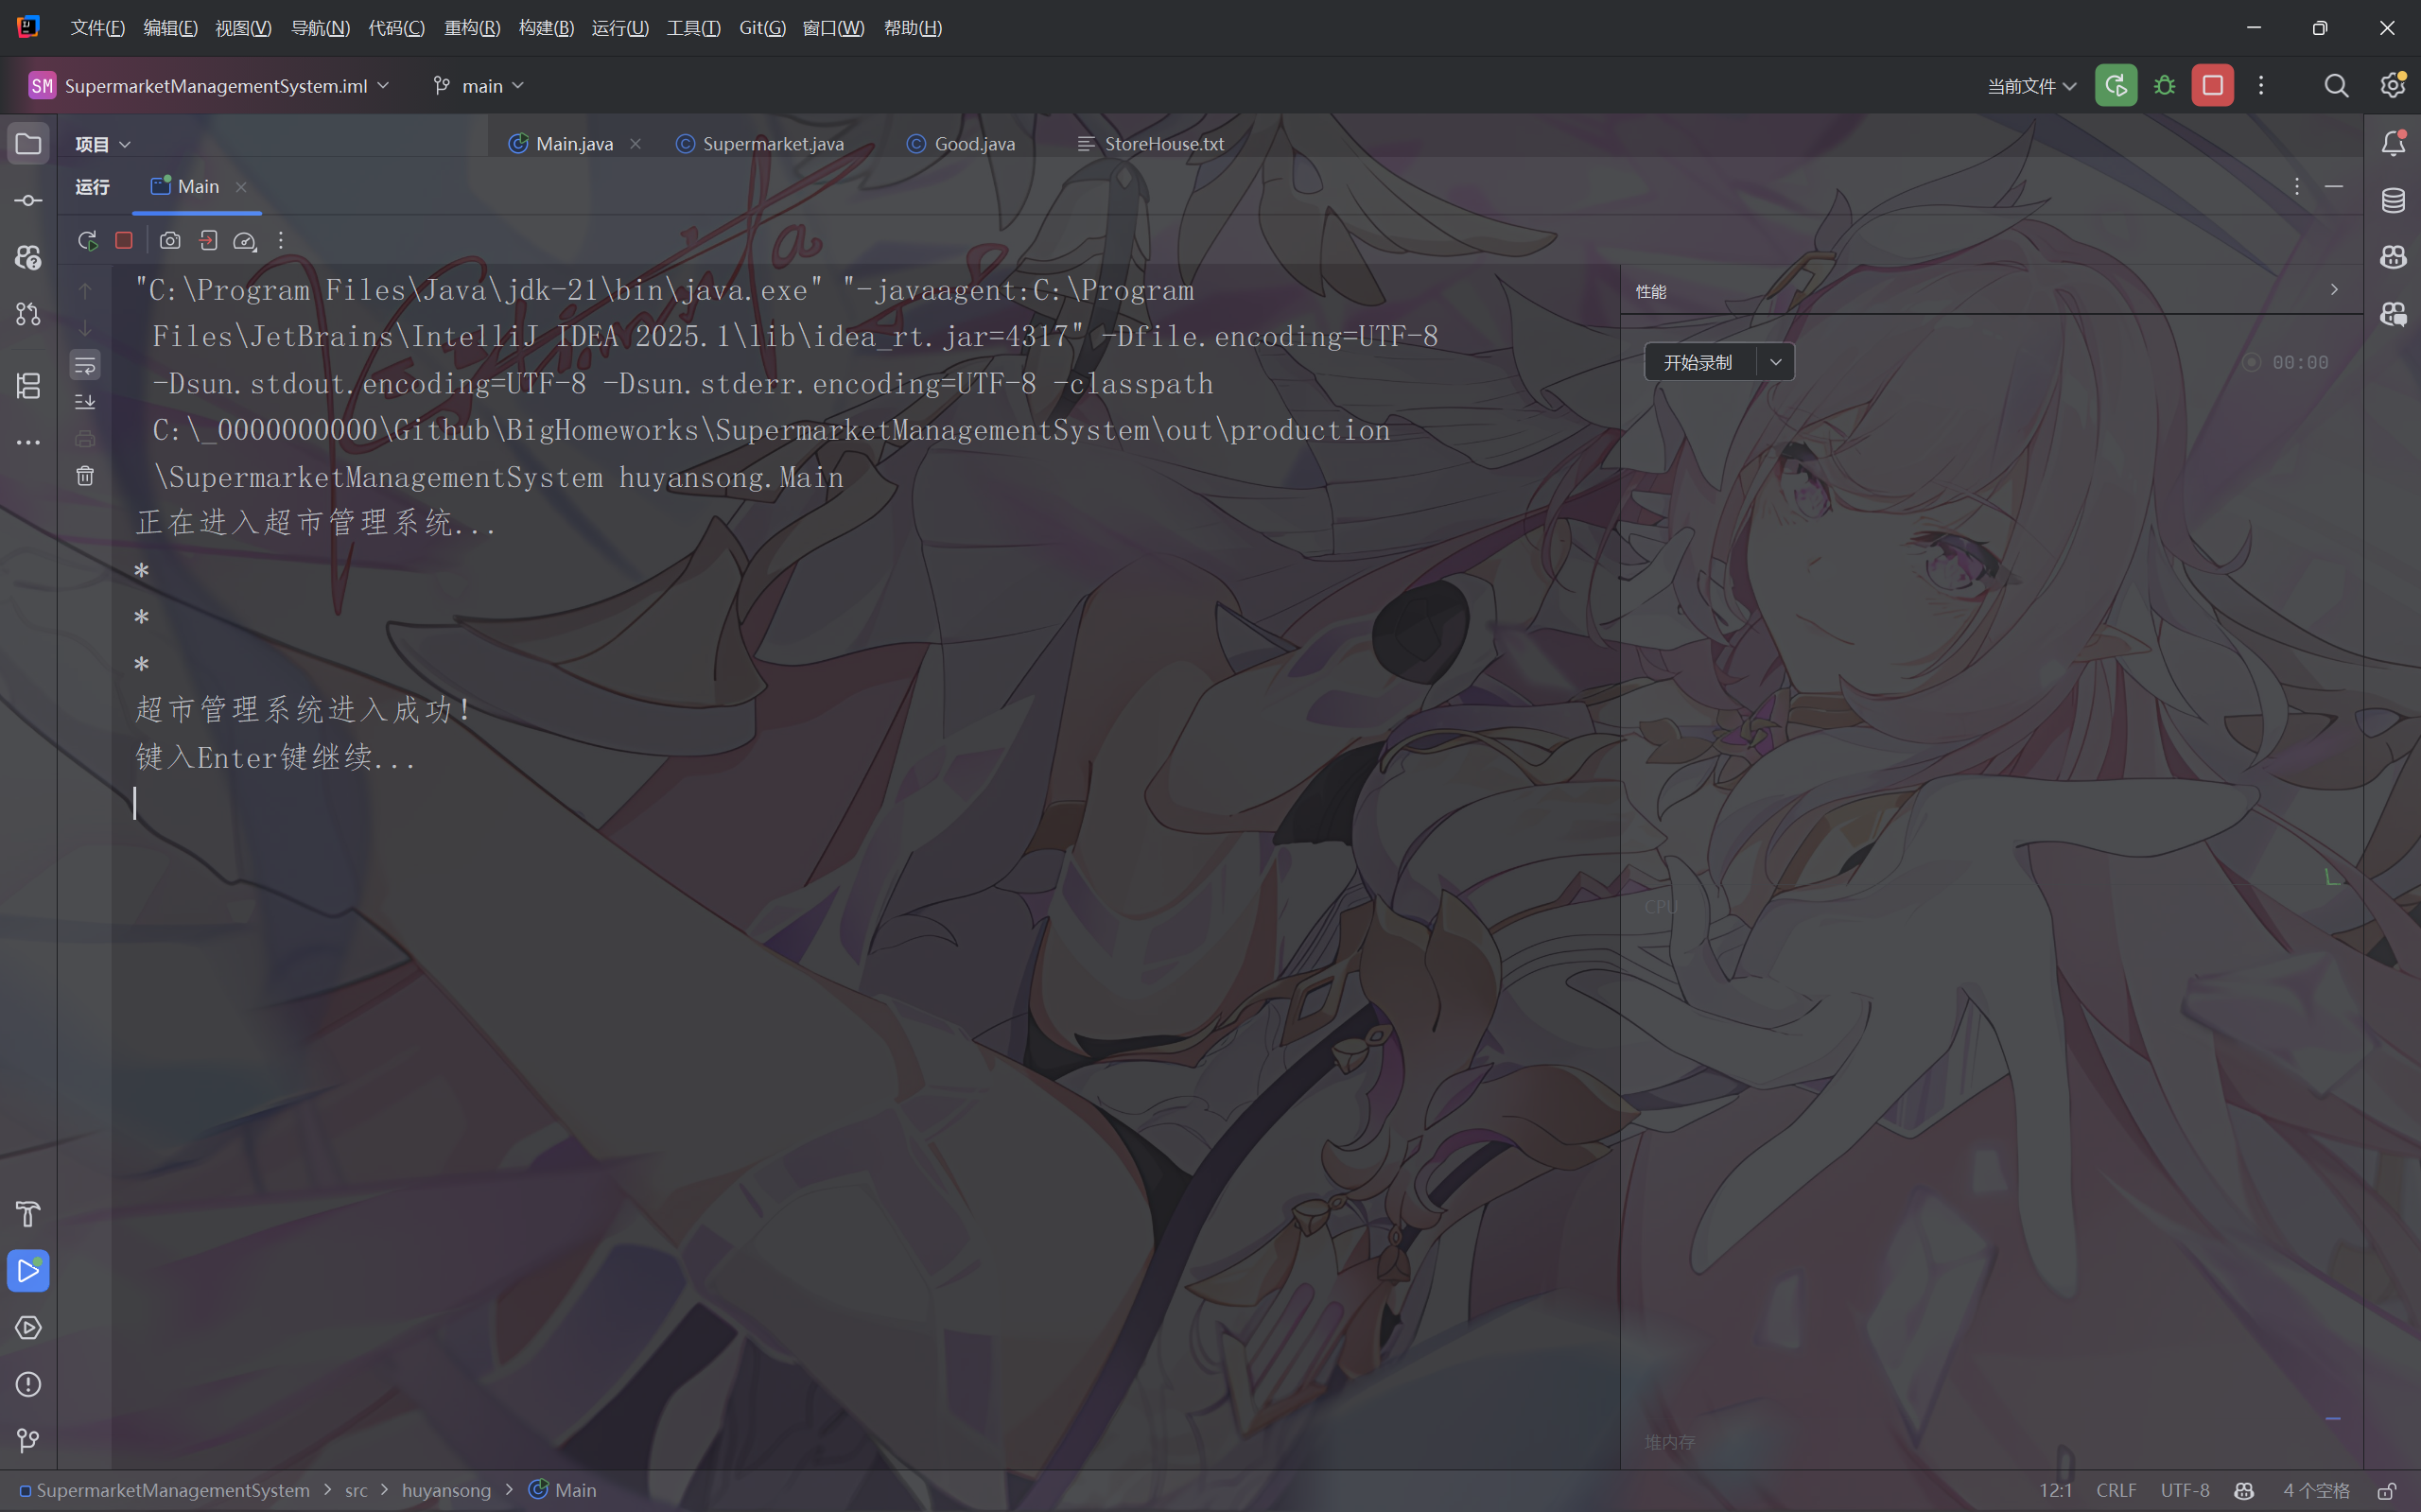
\includegraphics[width=\textwidth]{images/进入程序.png}
        \caption*{进入程序}
    \end{minipage}
    \hfill
    \begin{minipage}[t]{0.48\textwidth}
        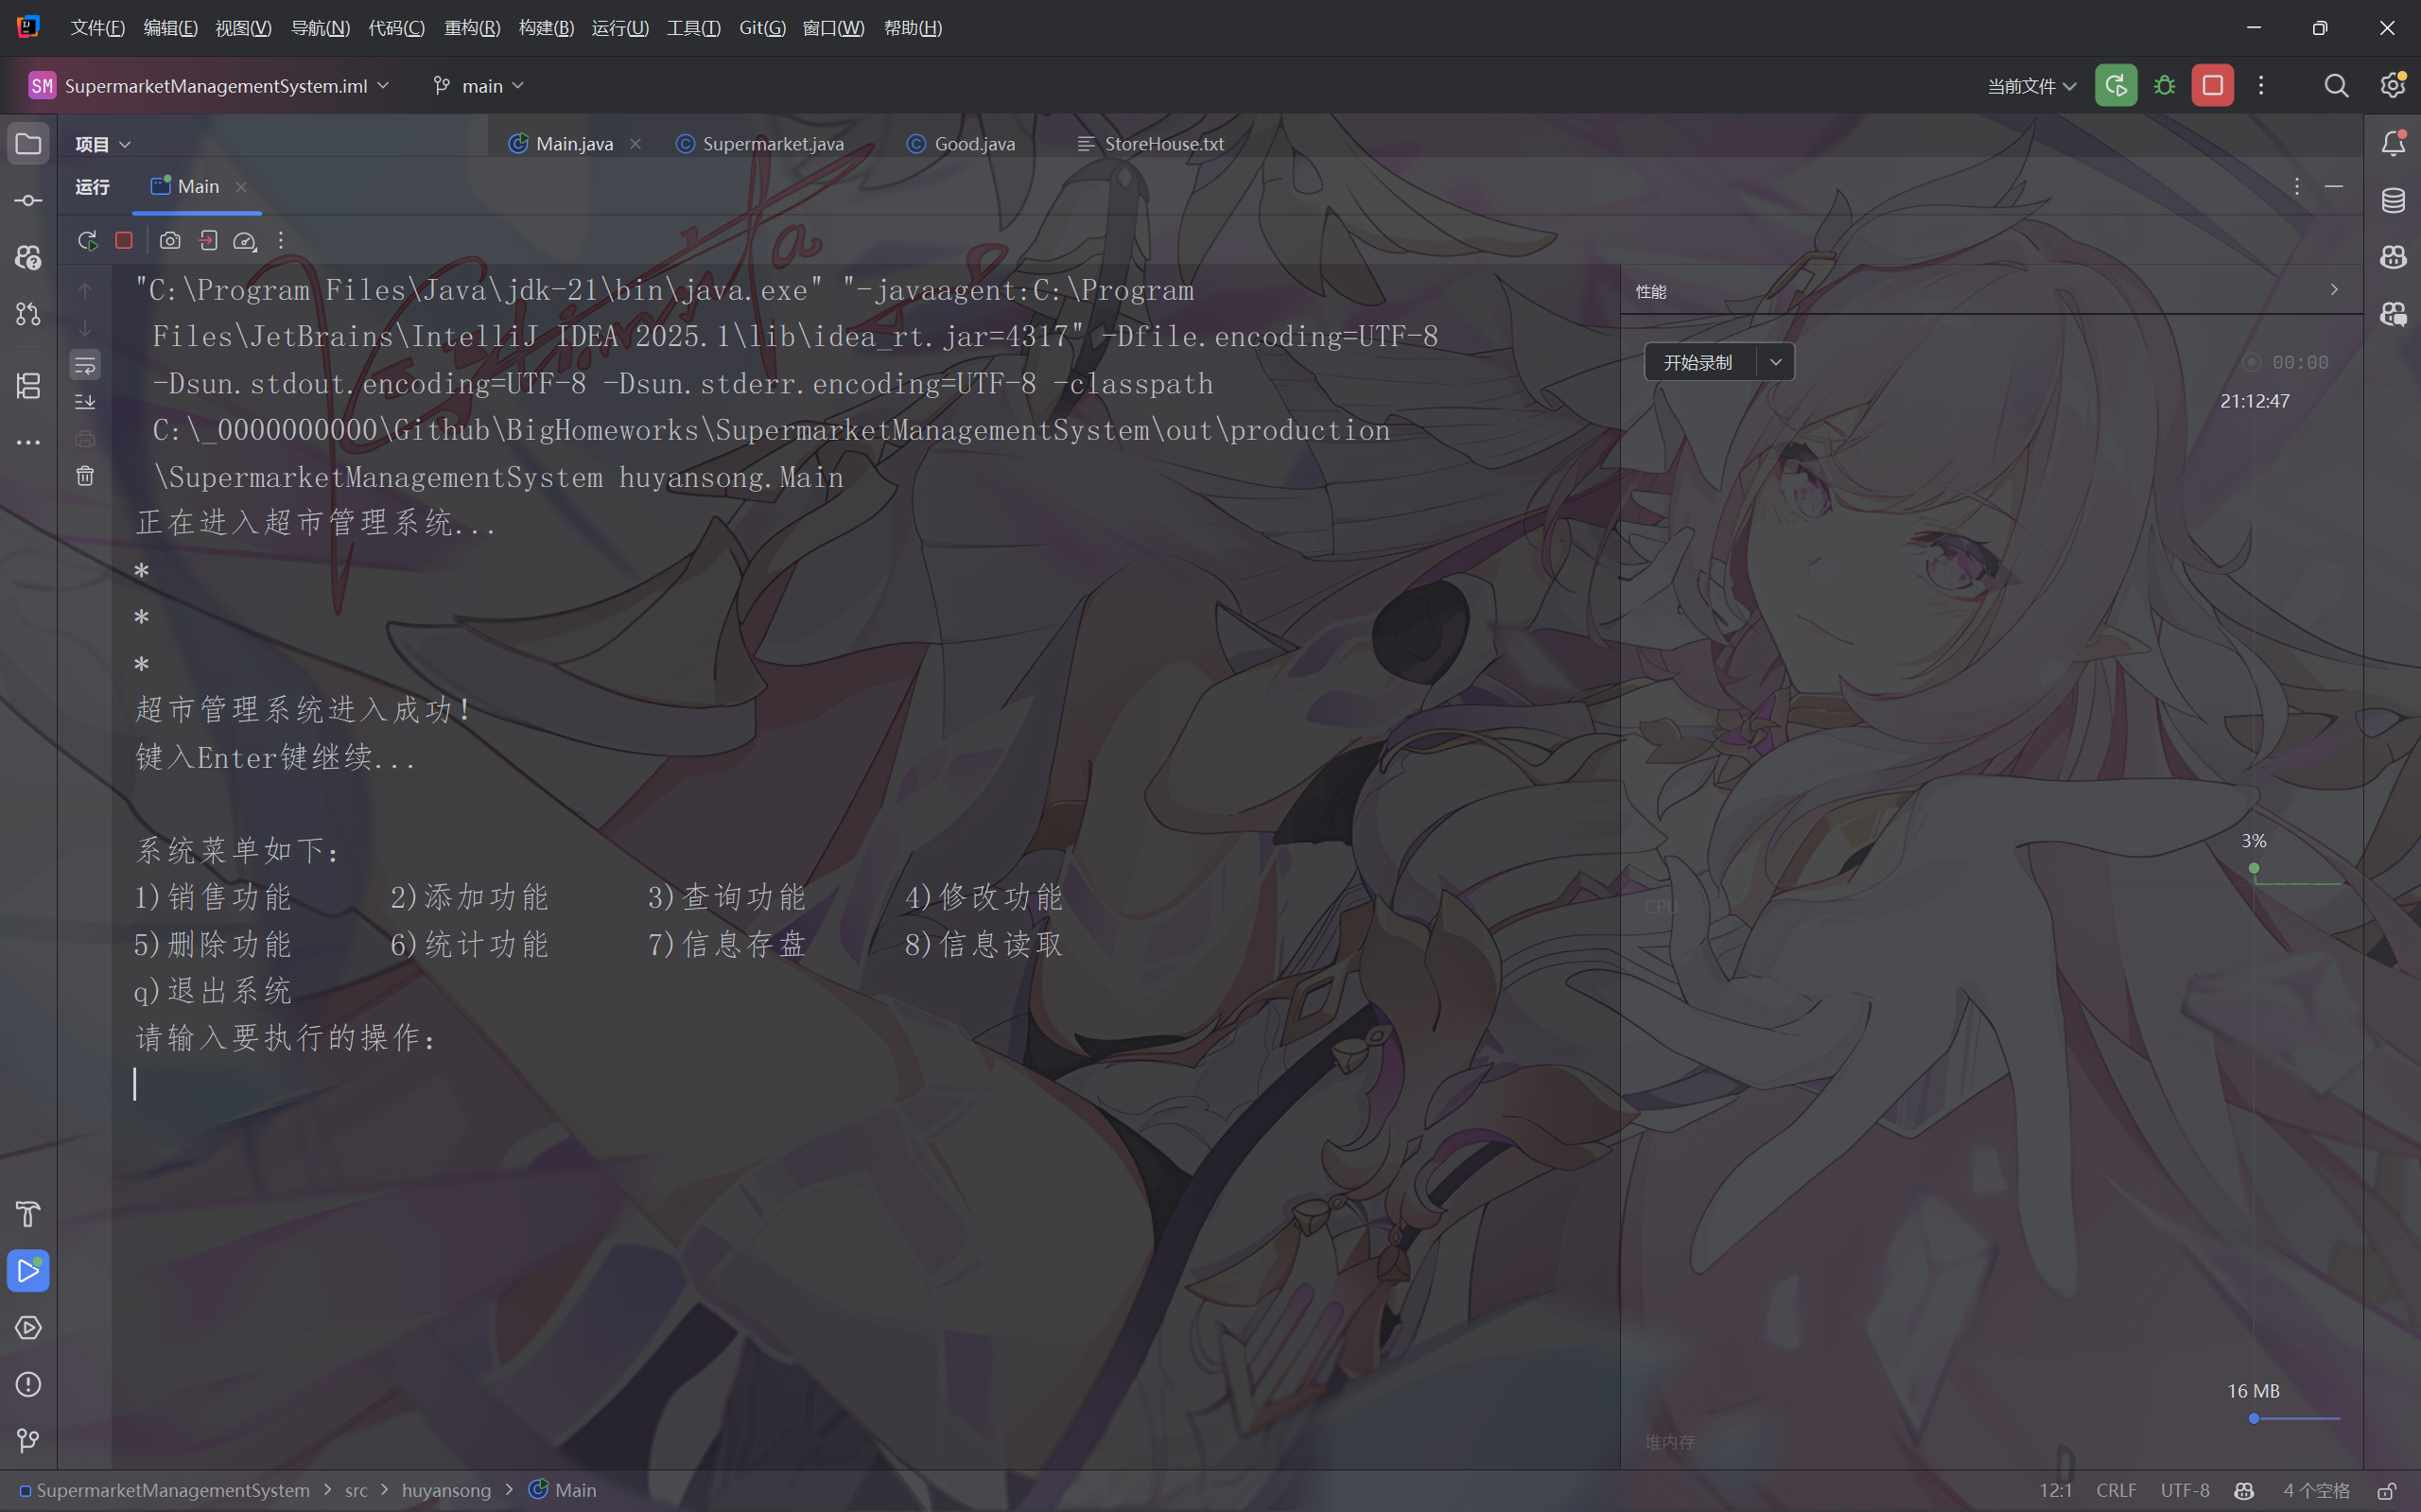
\includegraphics[width=\textwidth]{images/菜单显示.png}
        \caption*{菜单显示}
    \end{minipage}
\end{figure}

\begin{figure}[H]
    \begin{minipage}[t]{0.48\textwidth}
        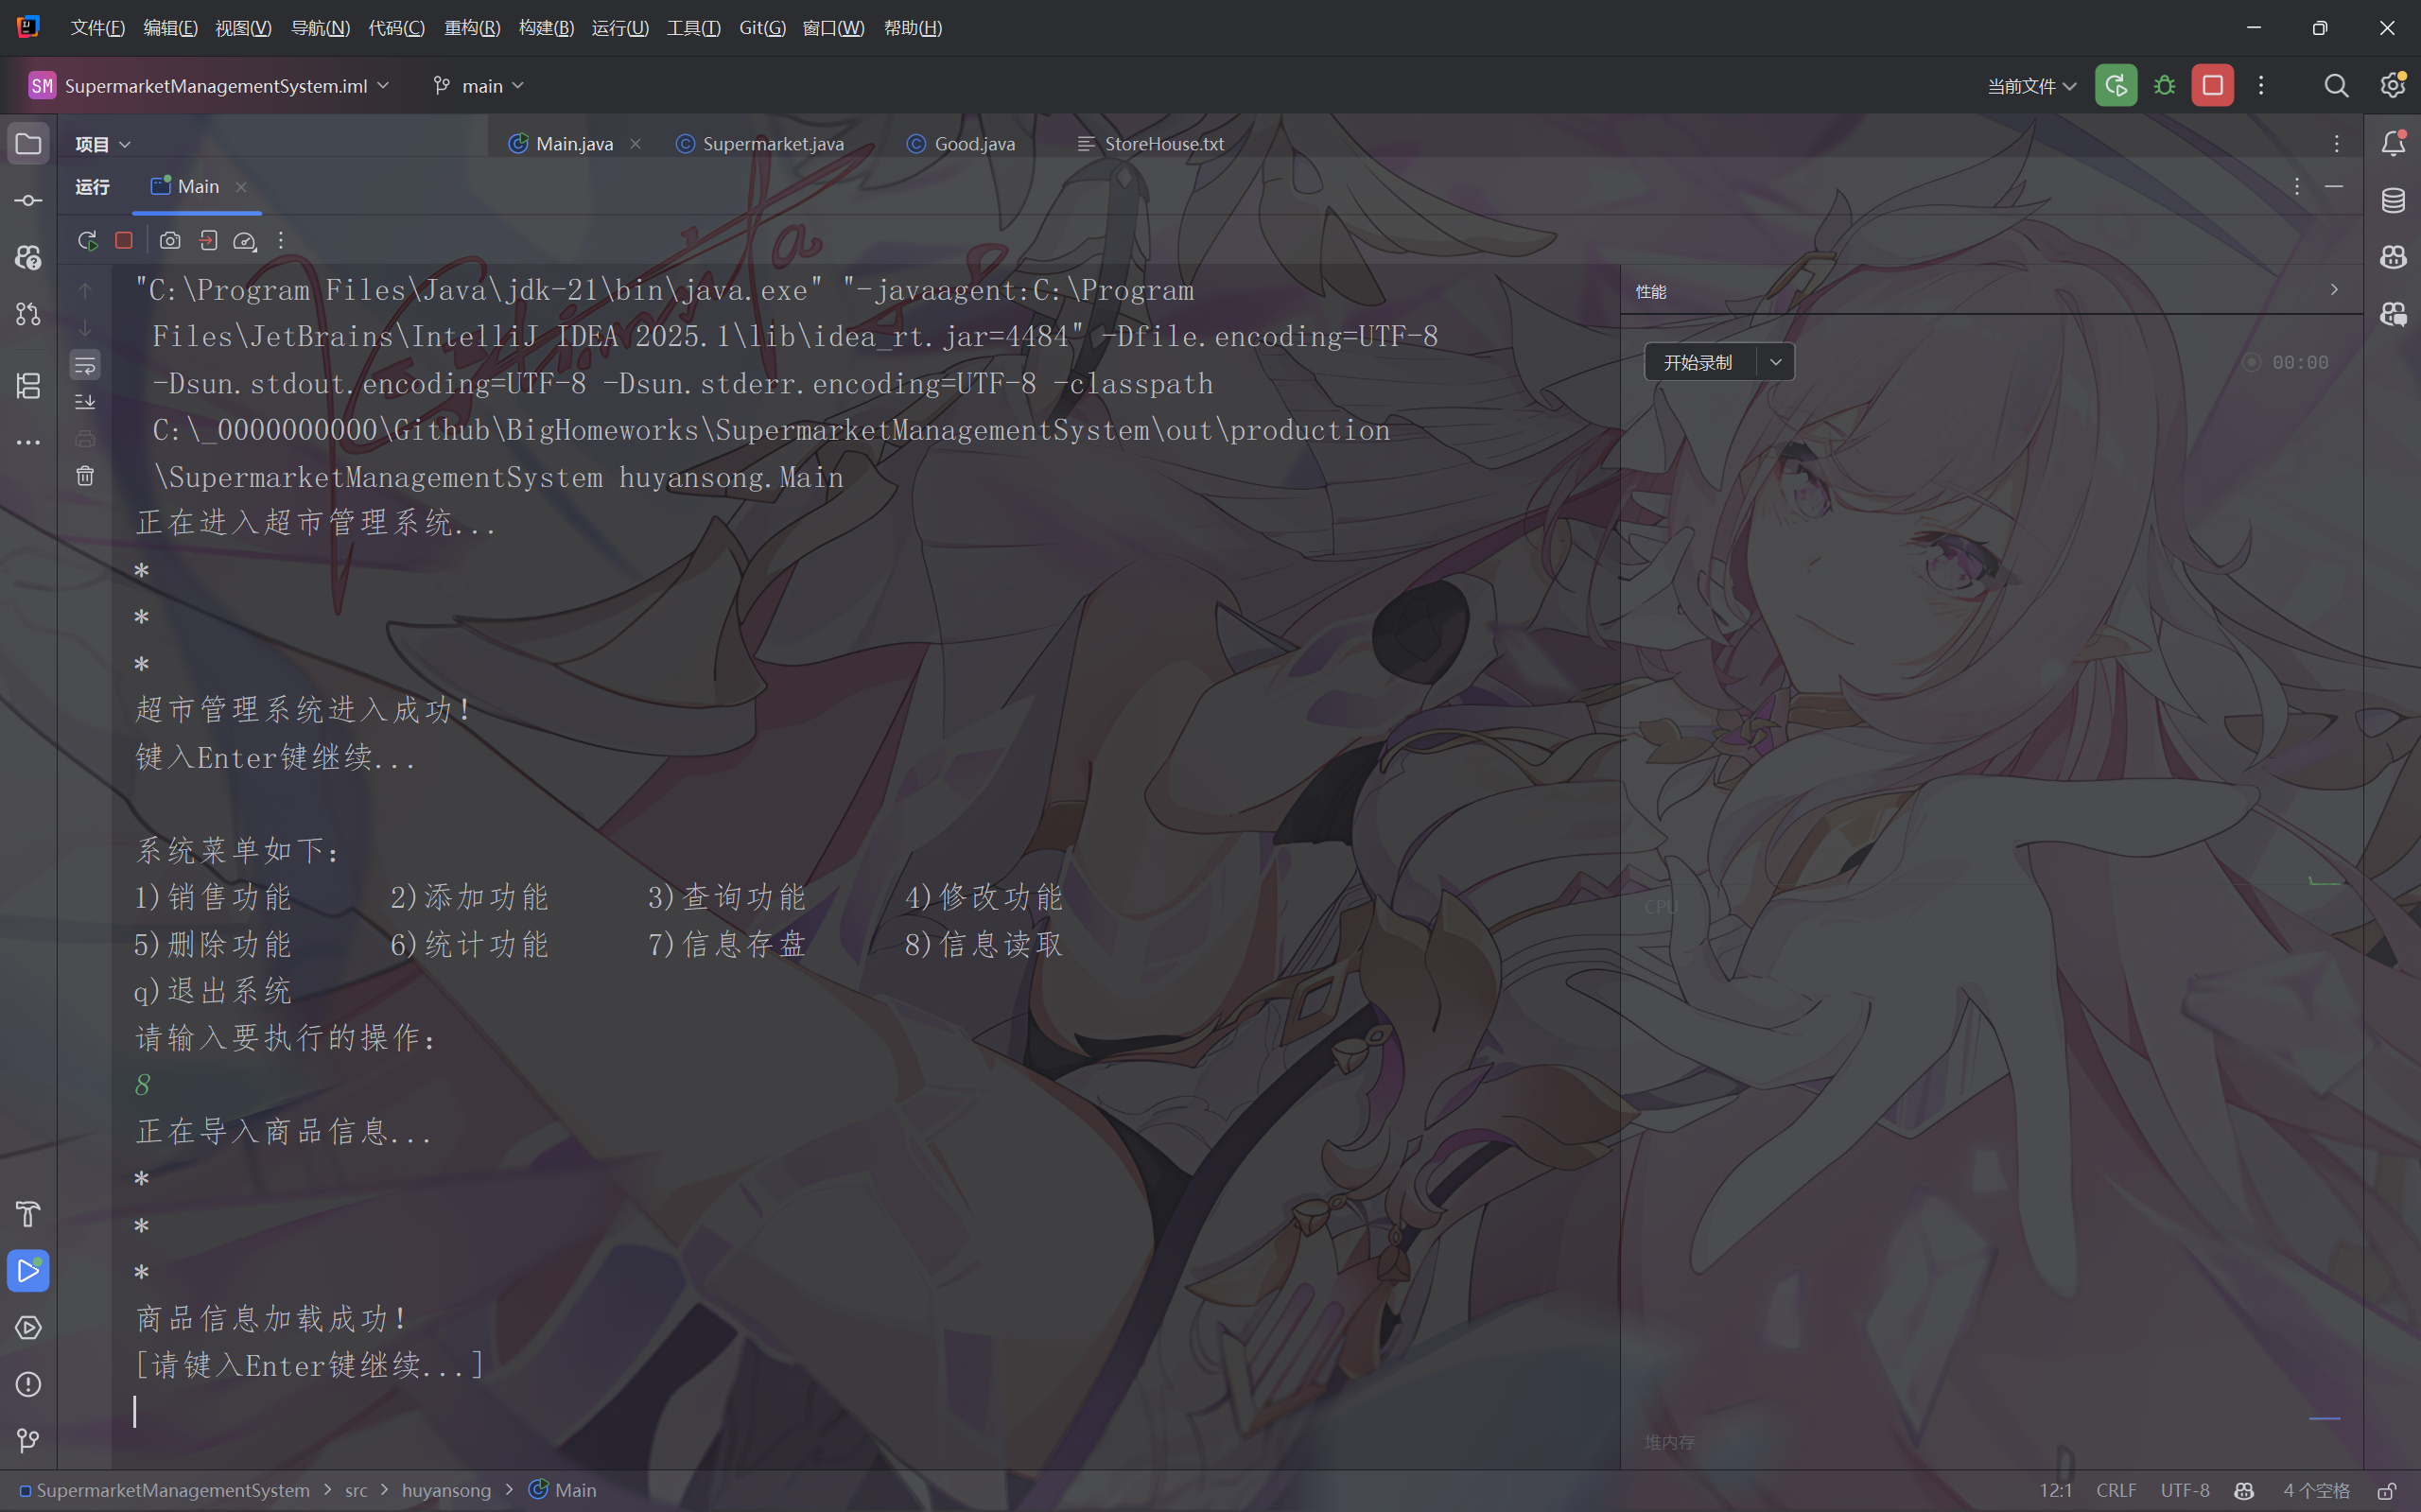
\includegraphics[width=\textwidth]{images/导入商品信息.png}
        \caption*{导入商品信息}
    \end{minipage}
    \hfill
    \begin{minipage}[t]{0.48\textwidth}
        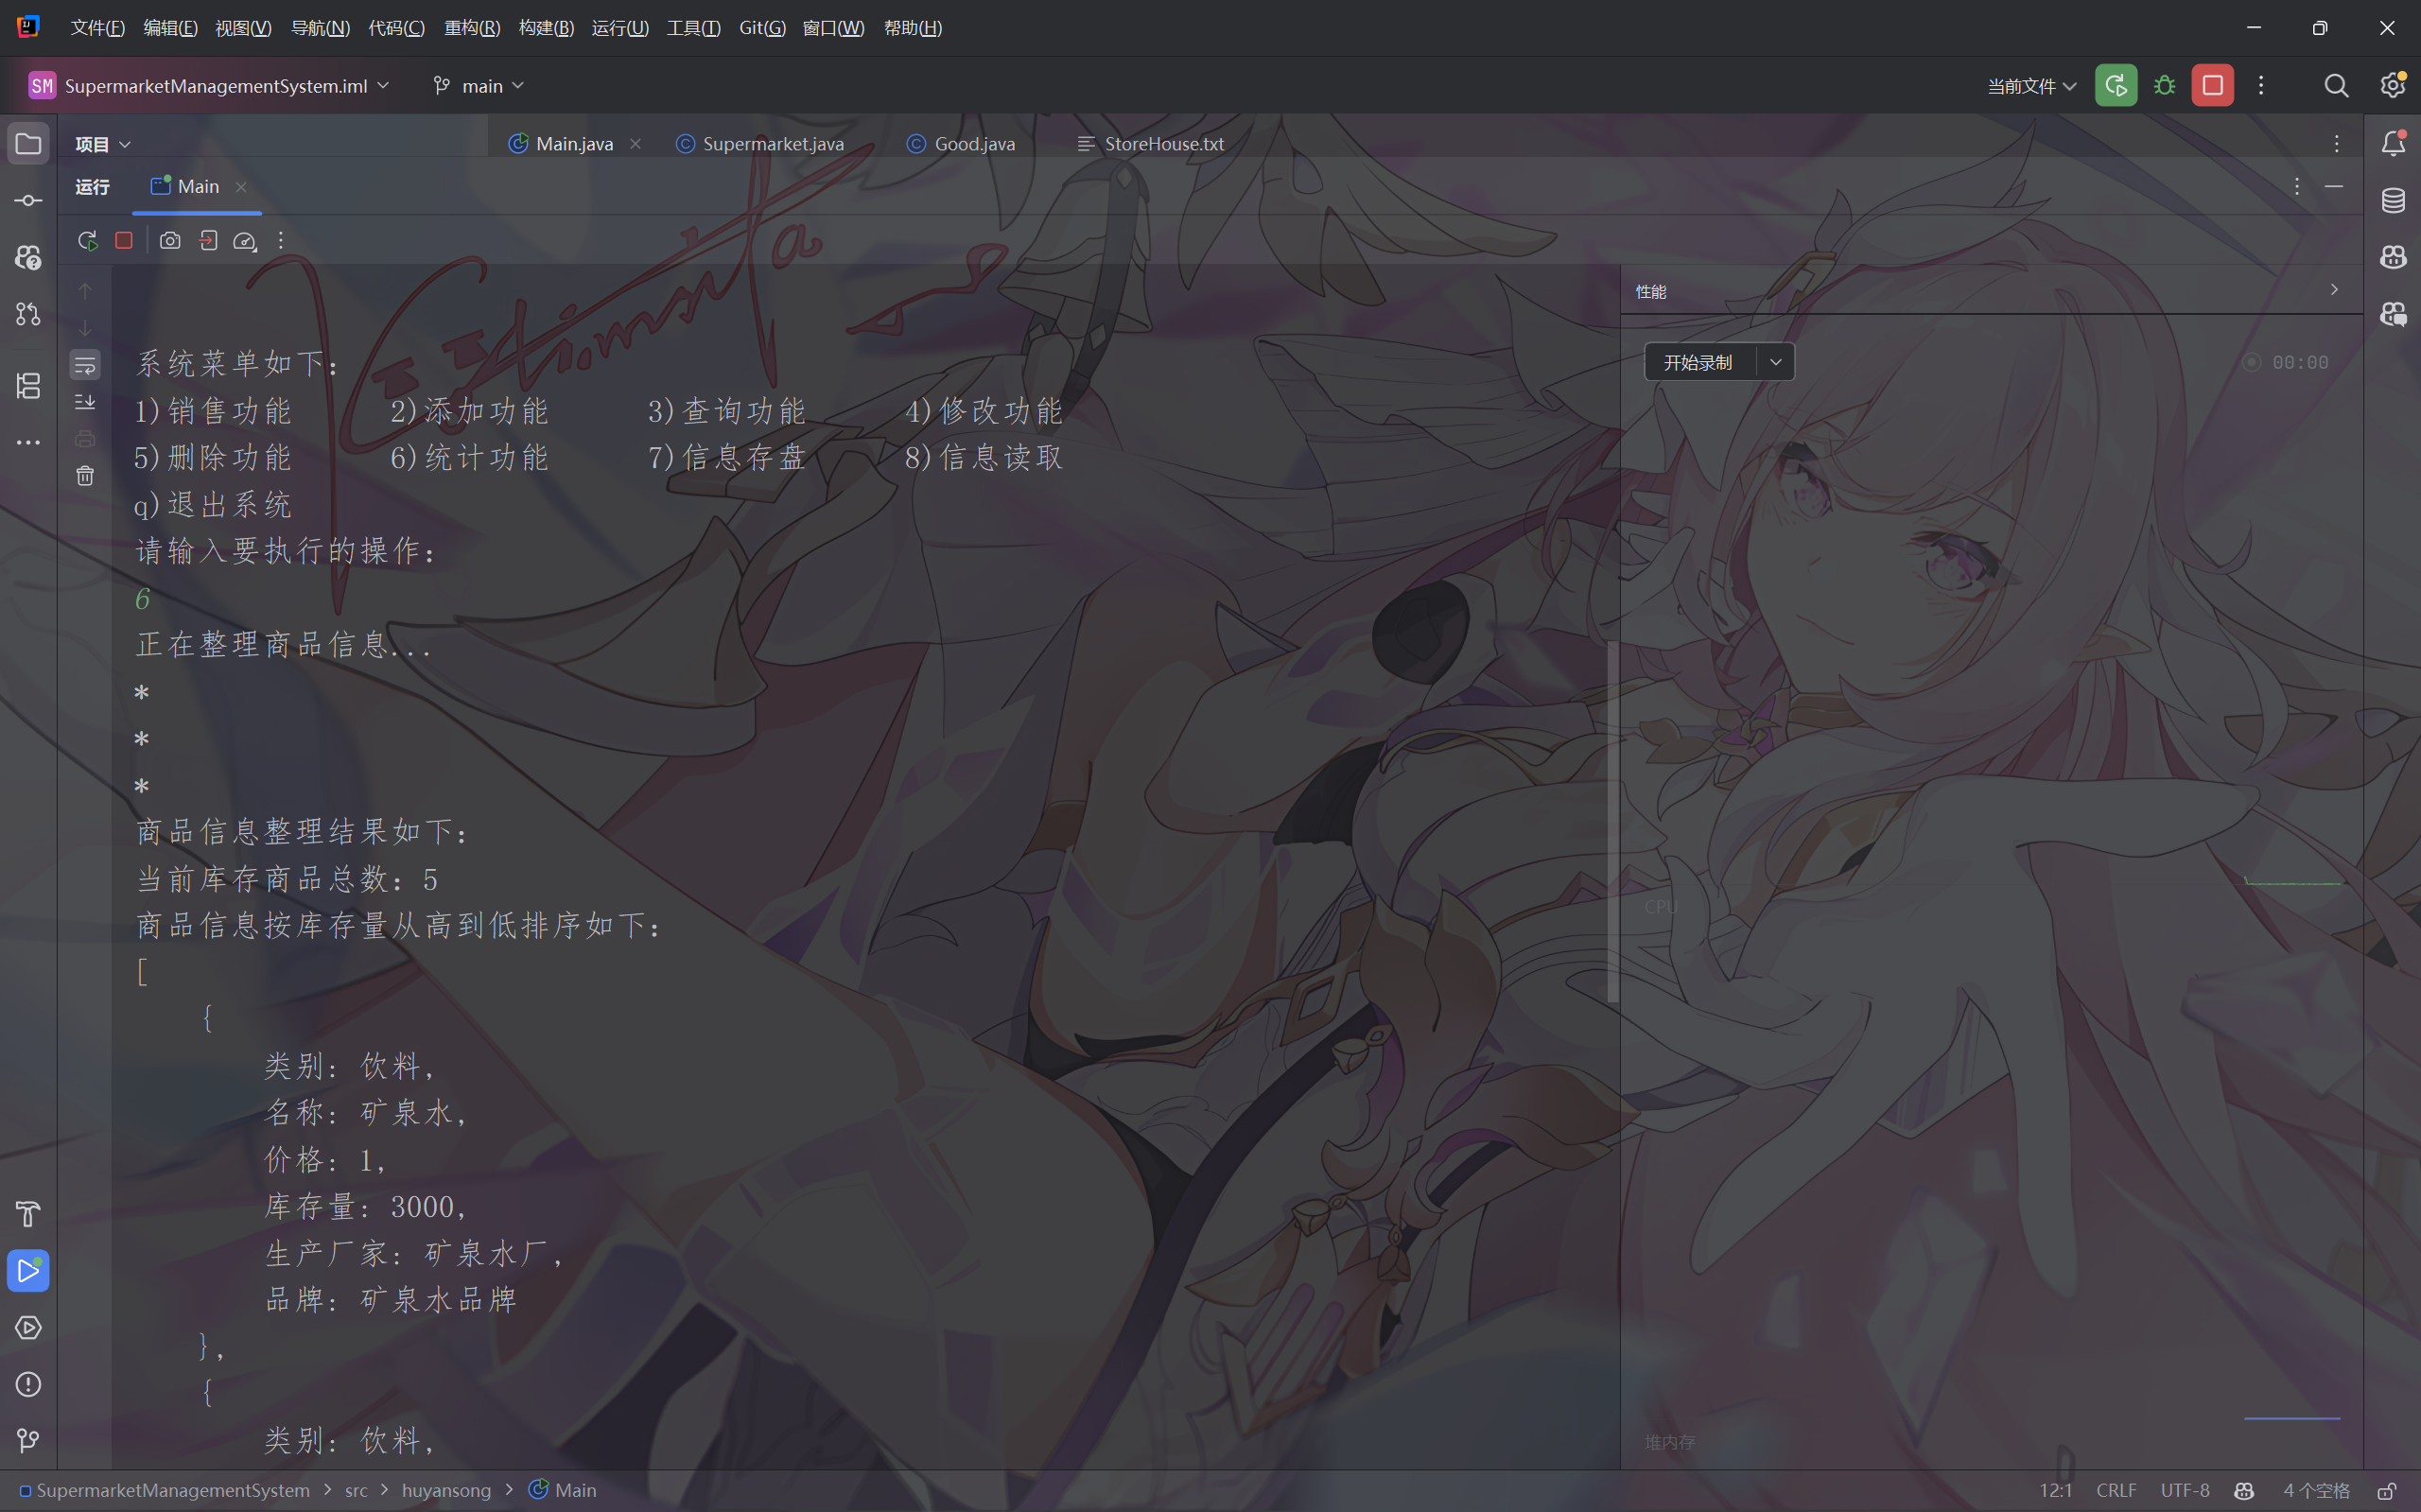
\includegraphics[width=\textwidth]{images/统计商品信息1.png}
        \caption*{统计商品信息1}
    \end{minipage}
\end{figure}

\begin{figure}[H]
    \begin{minipage}[t]{0.48\textwidth}
        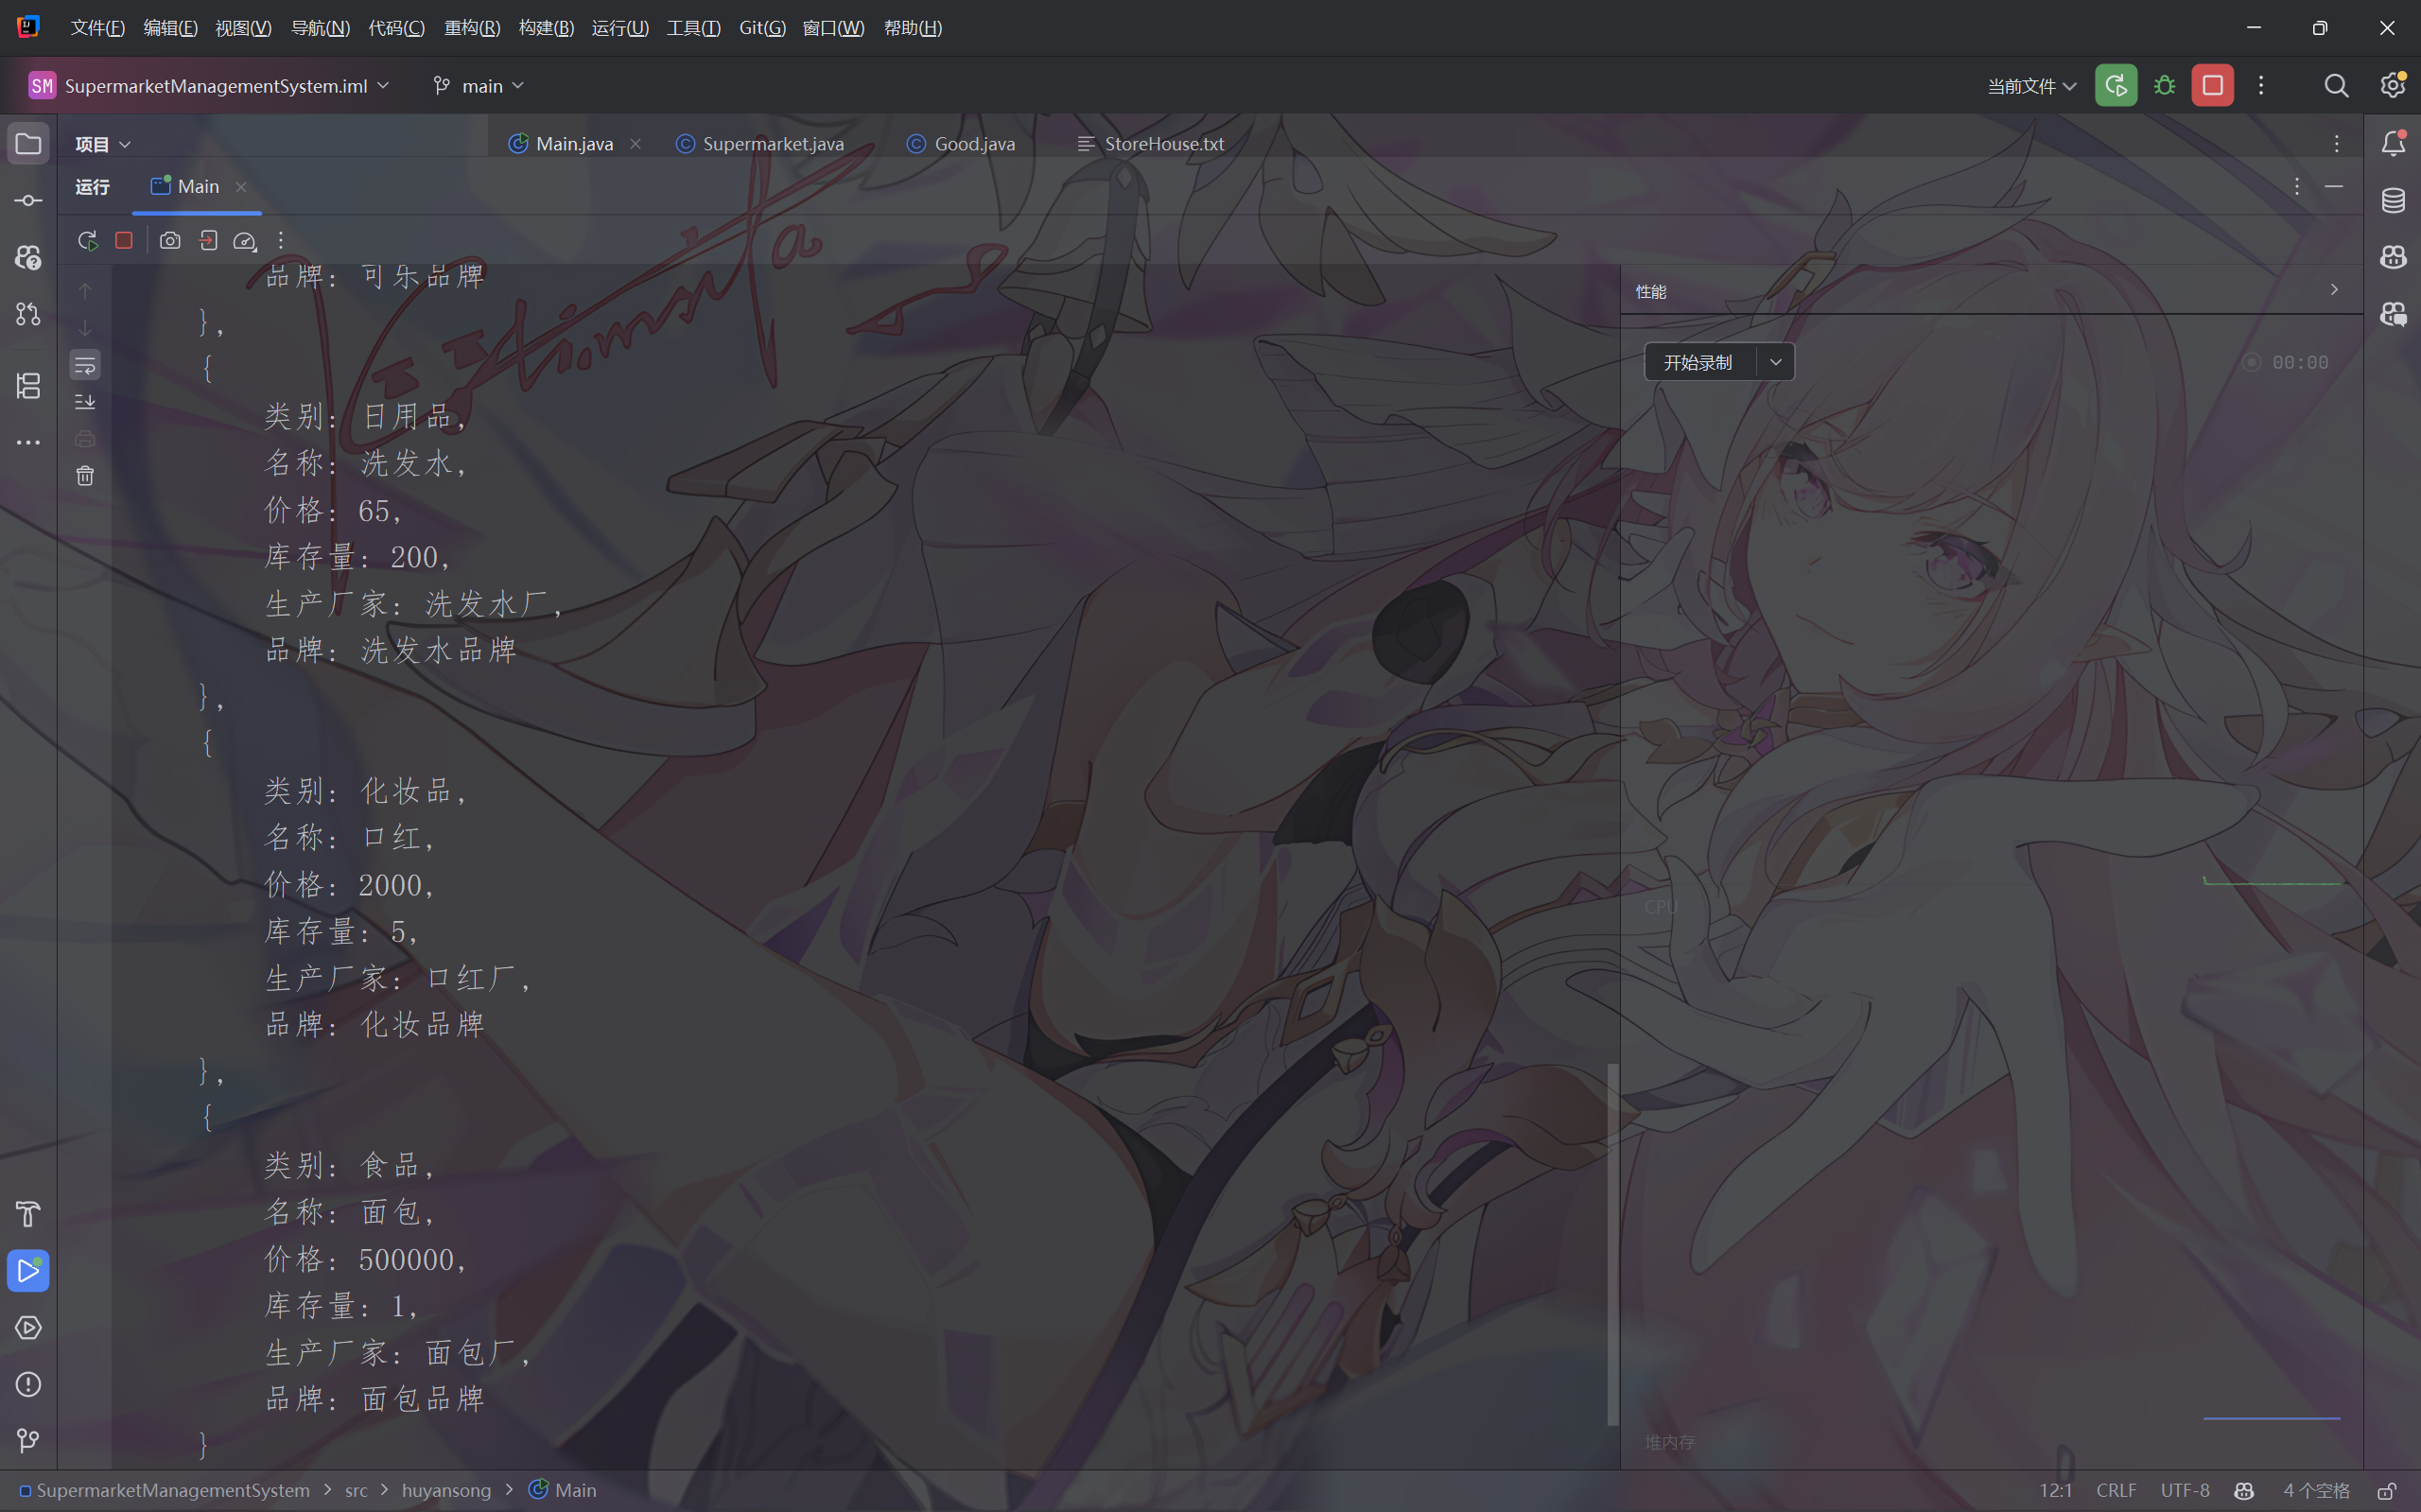
\includegraphics[width=\textwidth]{images/统计商品信息2.png}
        \caption*{统计商品信息2}
    \end{minipage}
    \hfill
    \begin{minipage}[t]{0.48\textwidth}
        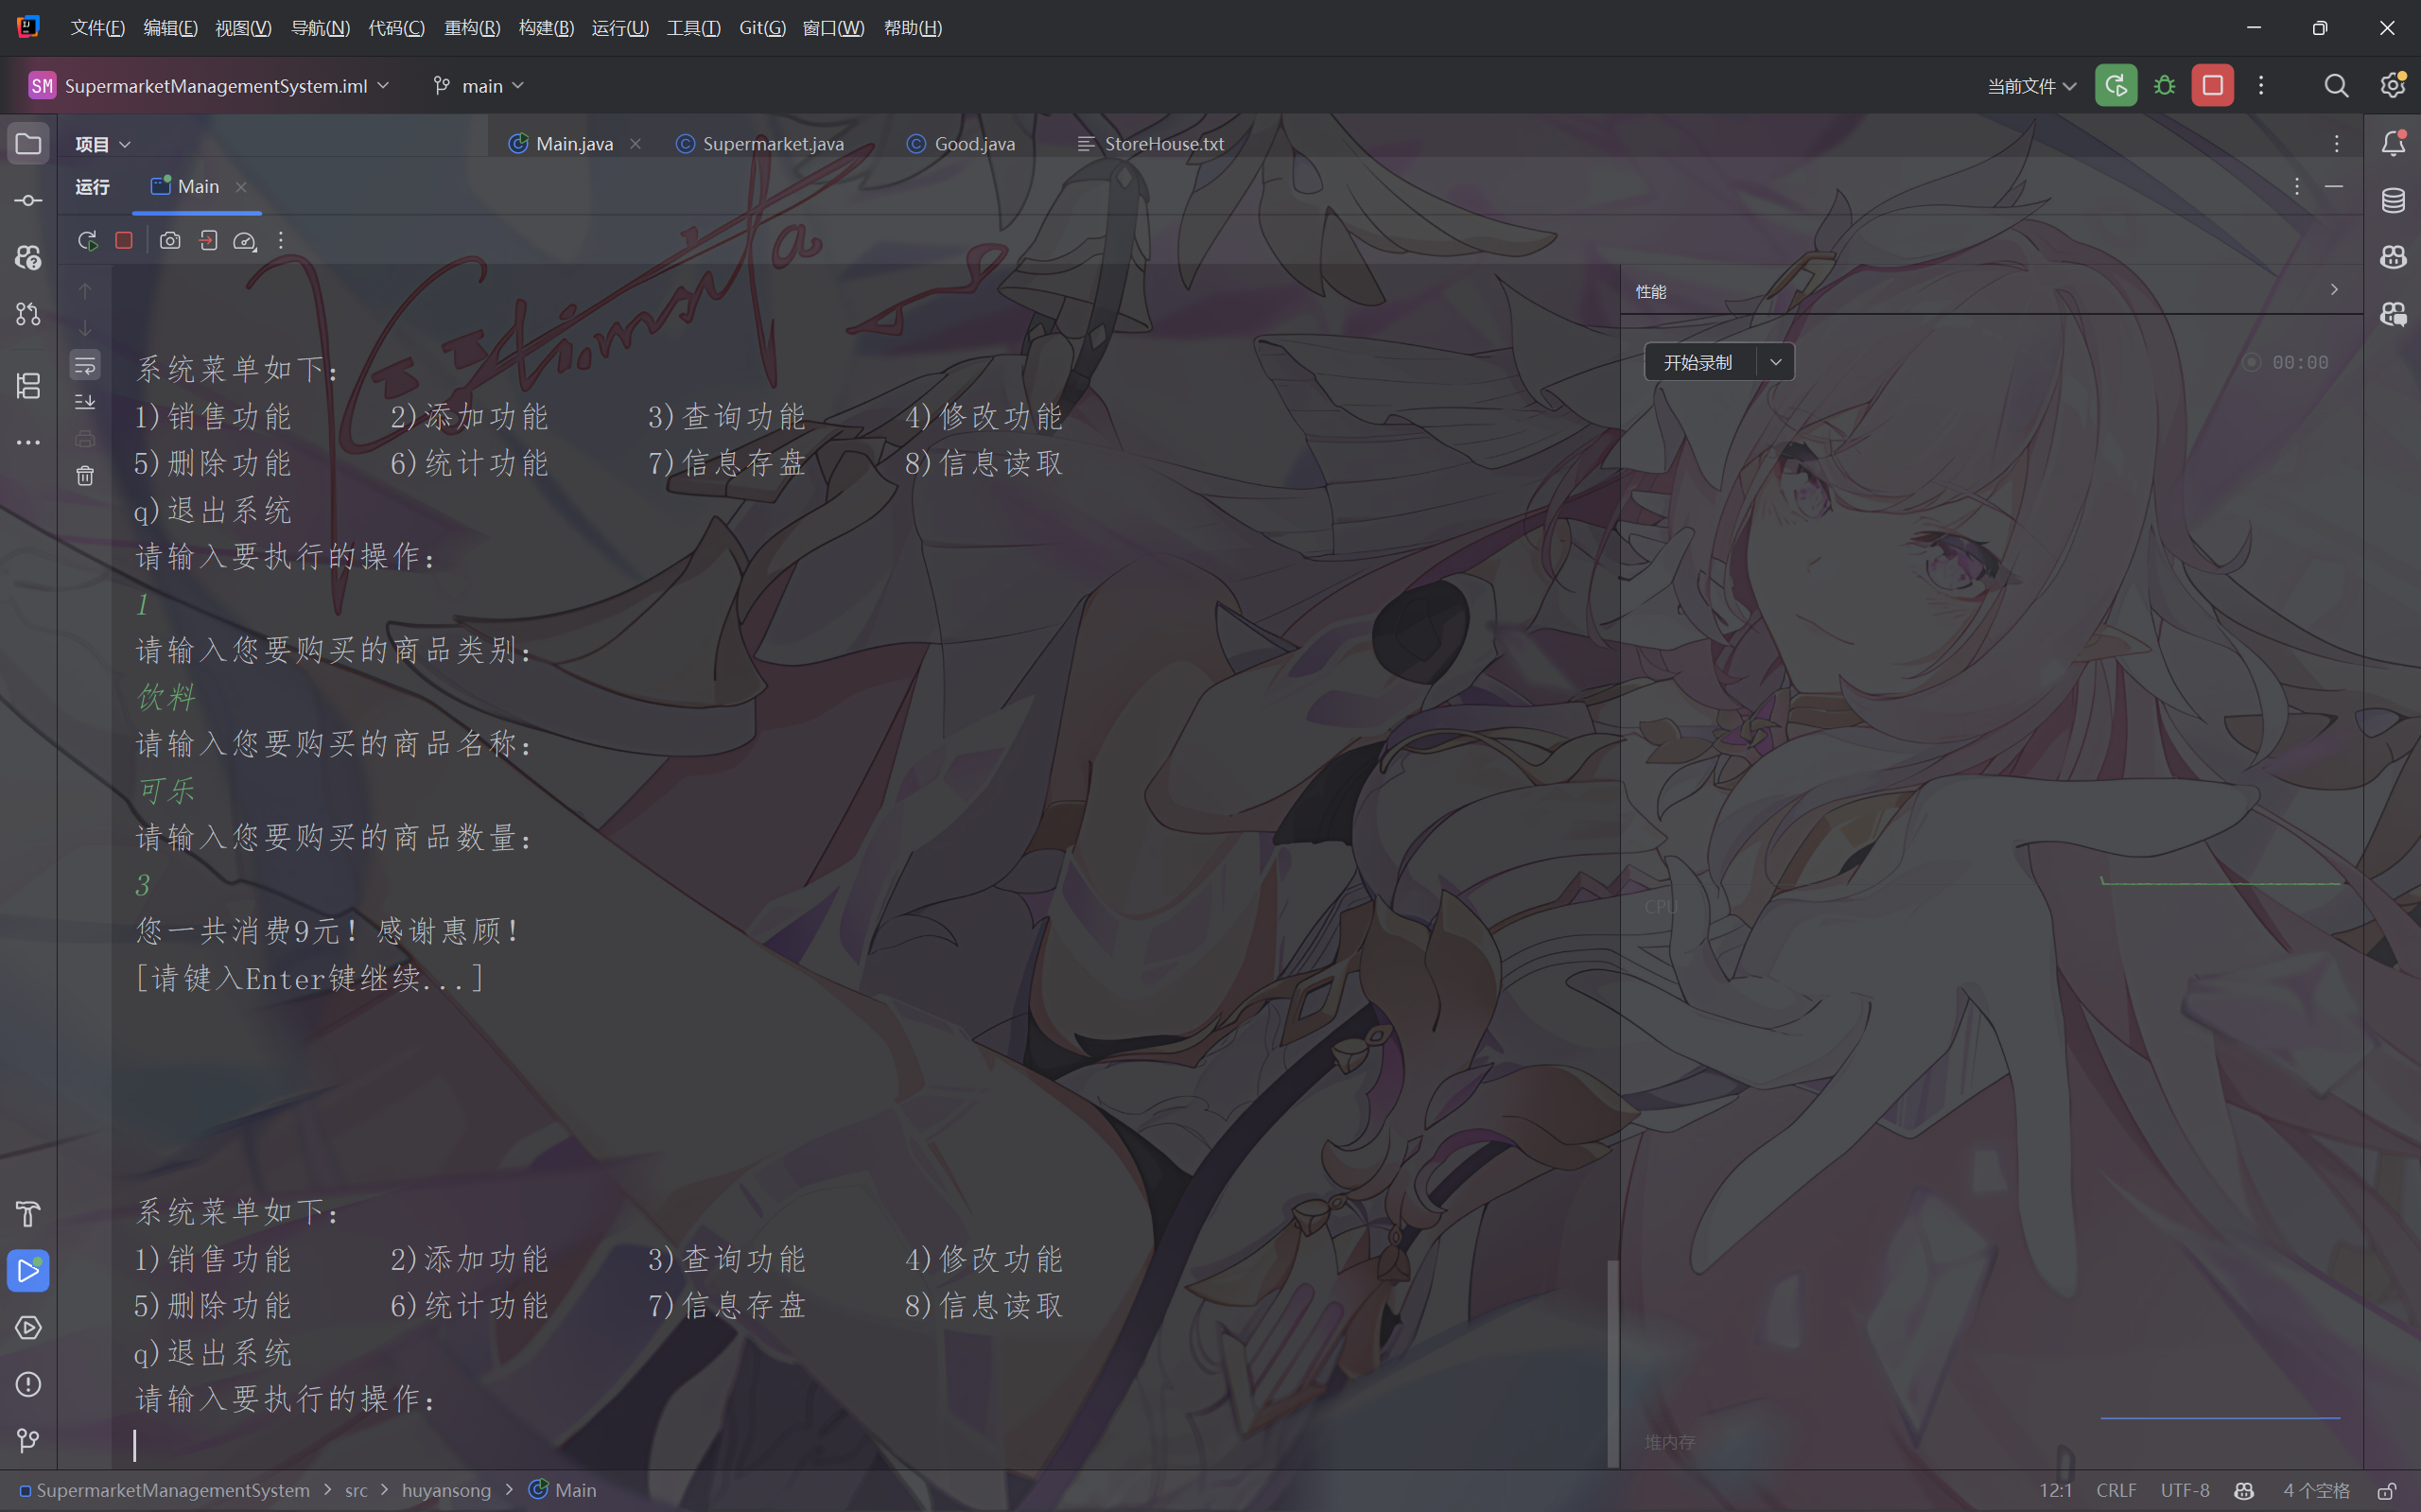
\includegraphics[width=\textwidth]{images/商品销售.png}
        \caption*{商品销售}
    \end{minipage}
\end{figure}

\begin{figure}[H]
    \begin{minipage}[t]{0.48\textwidth}
        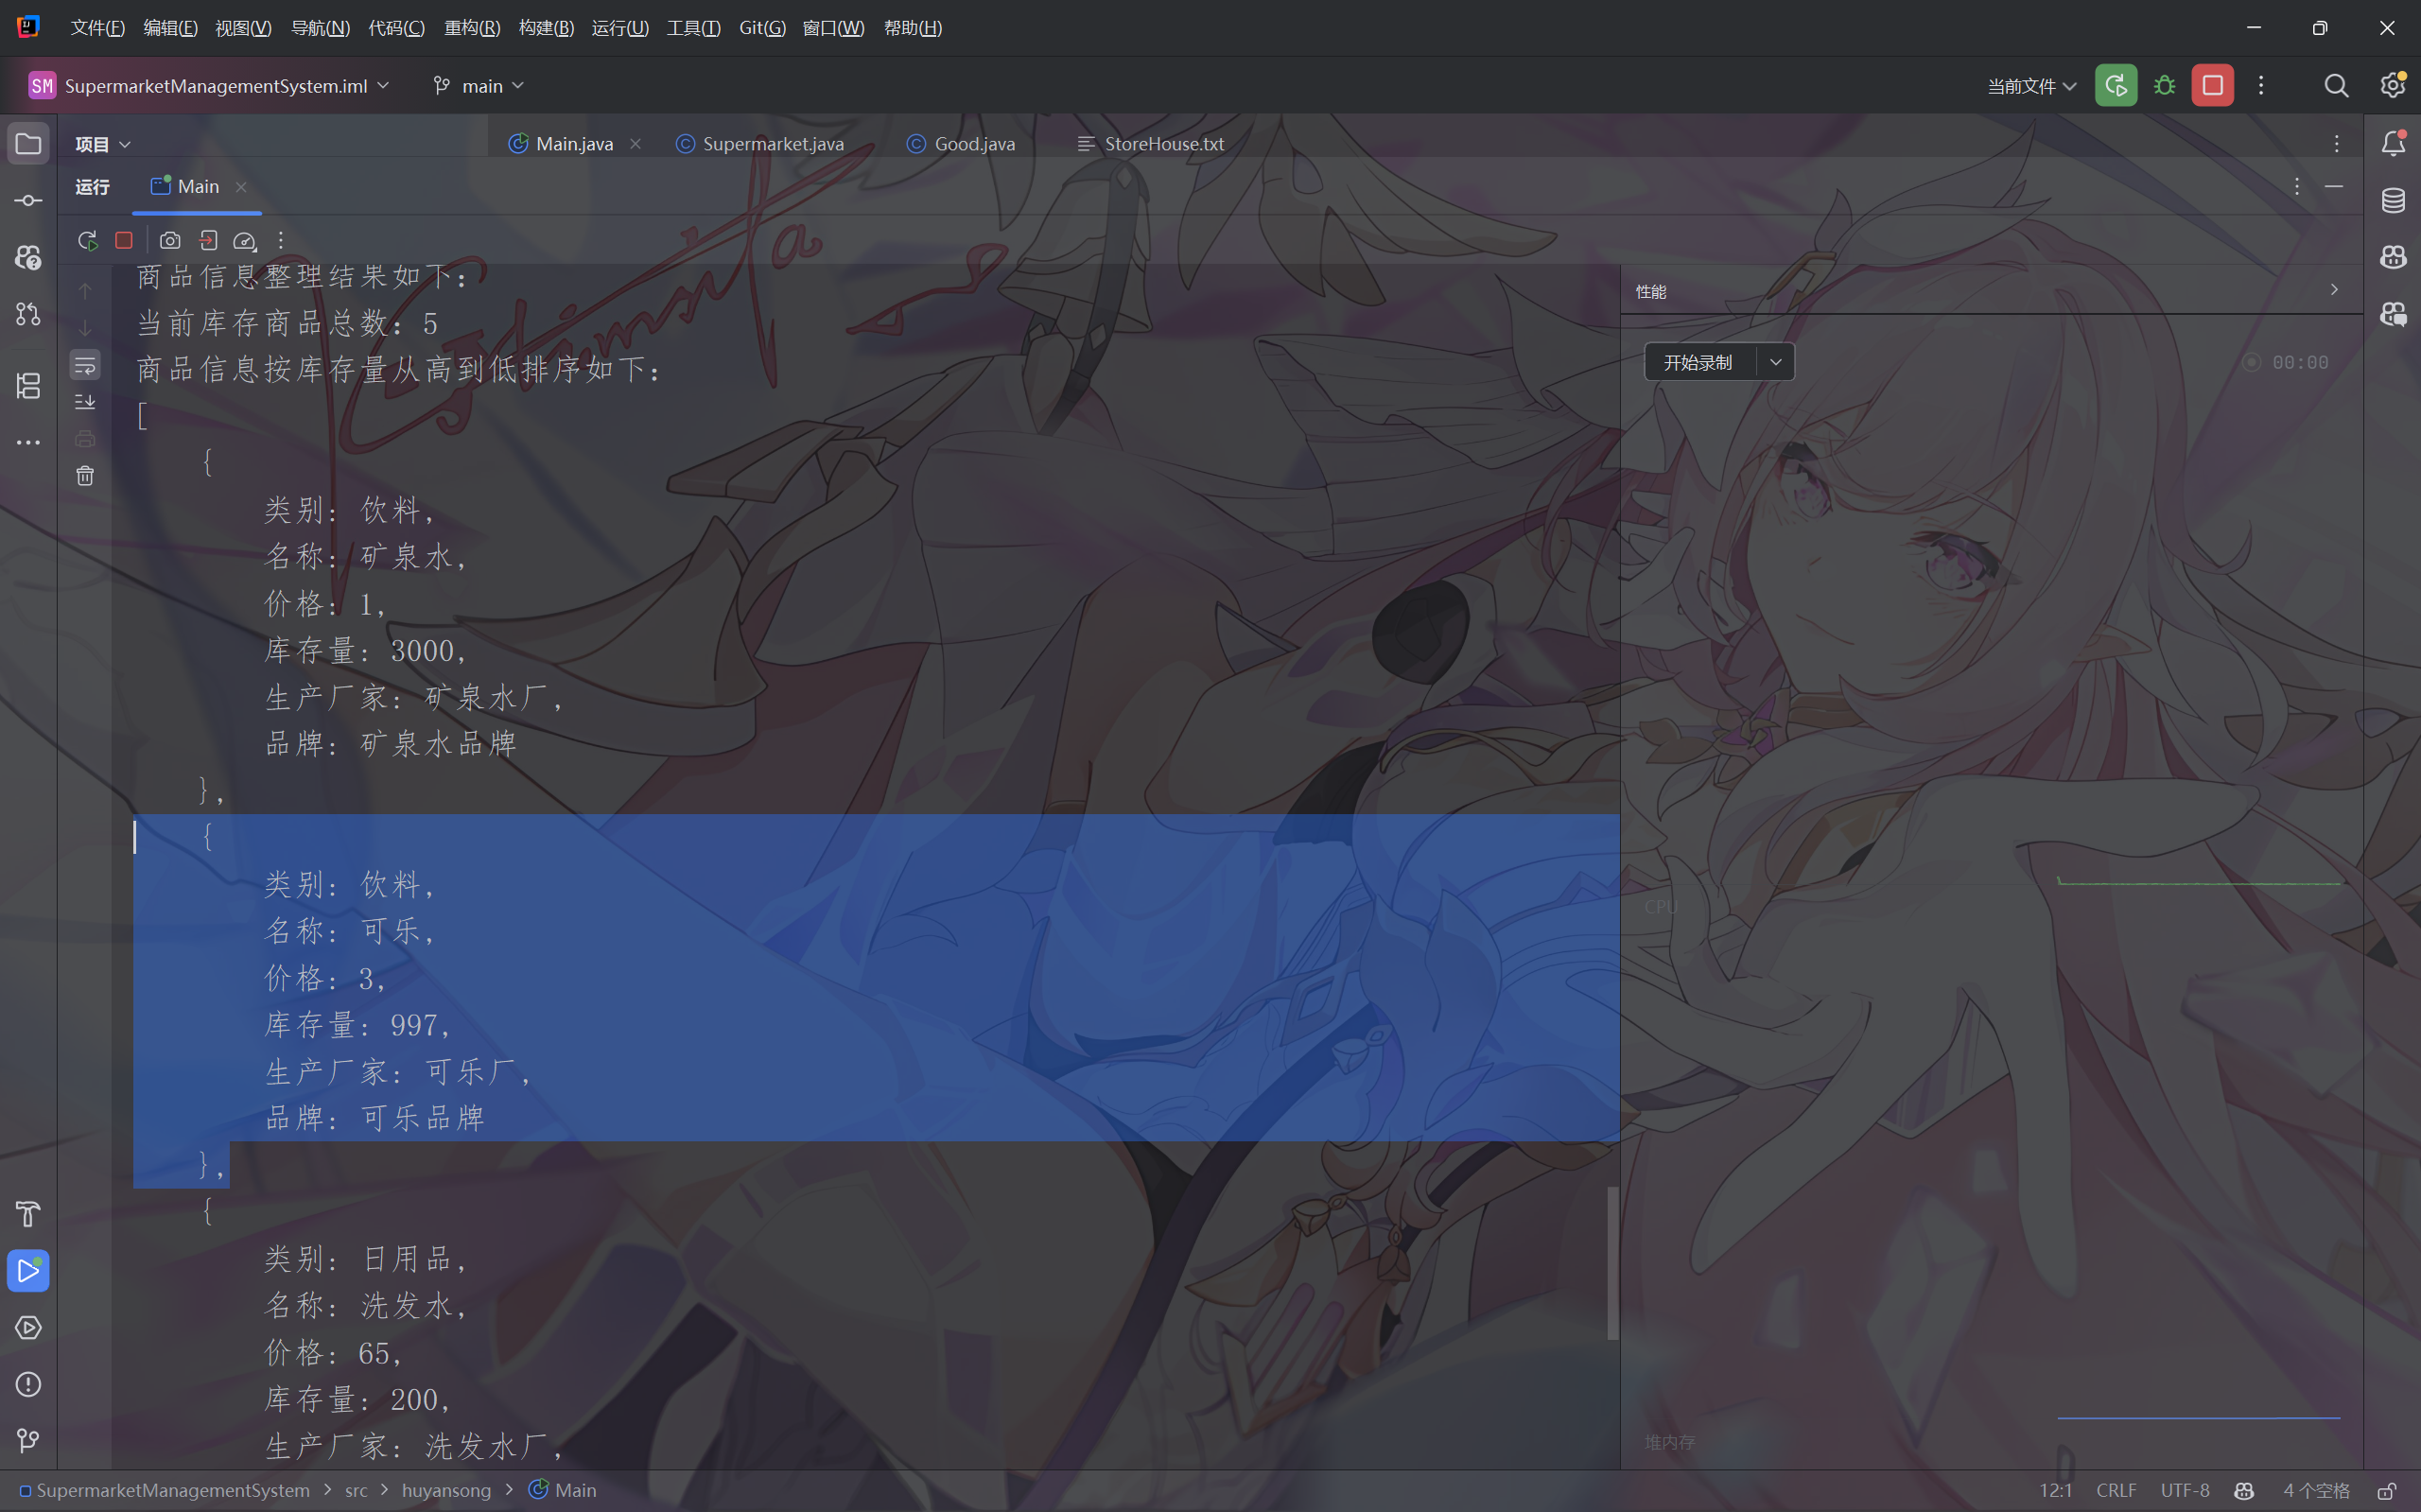
\includegraphics[width=\textwidth]{images/销售商品时库存信息随之改变.png}
        \caption*{销售商品时库存信息随之改变}
    \end{minipage}
    \hfill
    \begin{minipage}[t]{0.48\textwidth}
        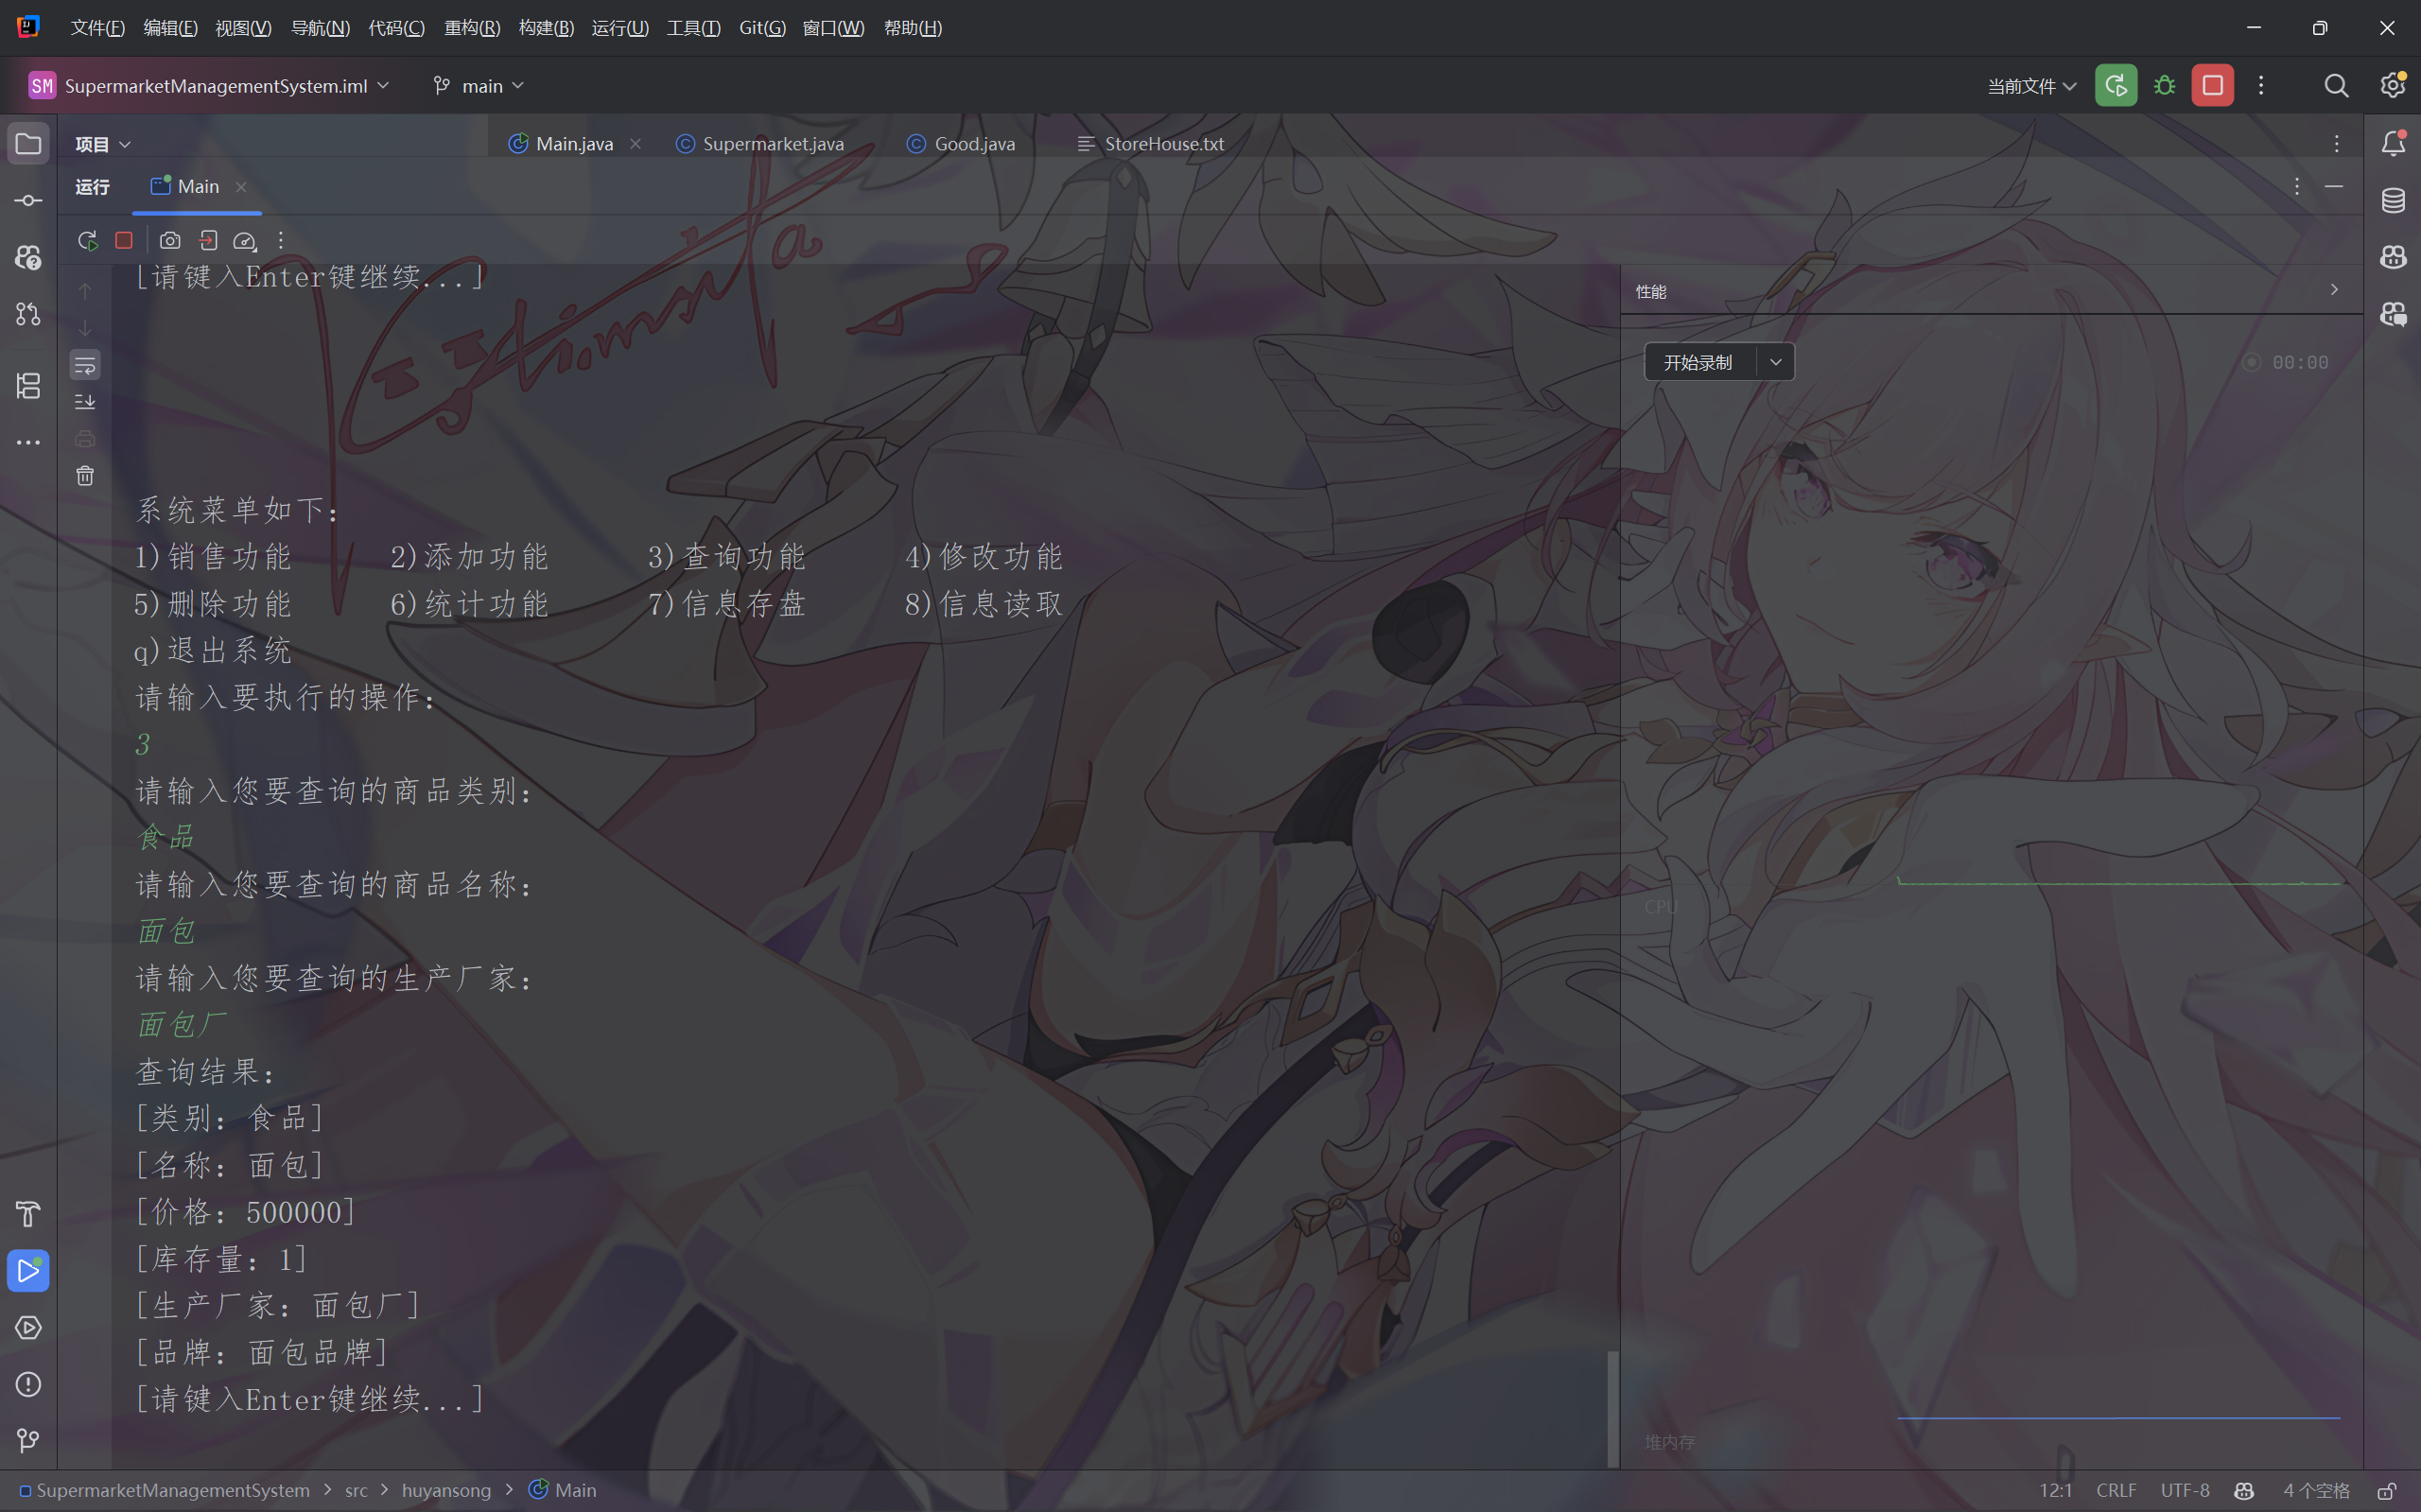
\includegraphics[width=\textwidth]{images/查询商品.png}
        \caption*{查询商品}
    \end{minipage}
\end{figure}

\begin{figure}[H]
    \begin{minipage}[t]{0.48\textwidth}
        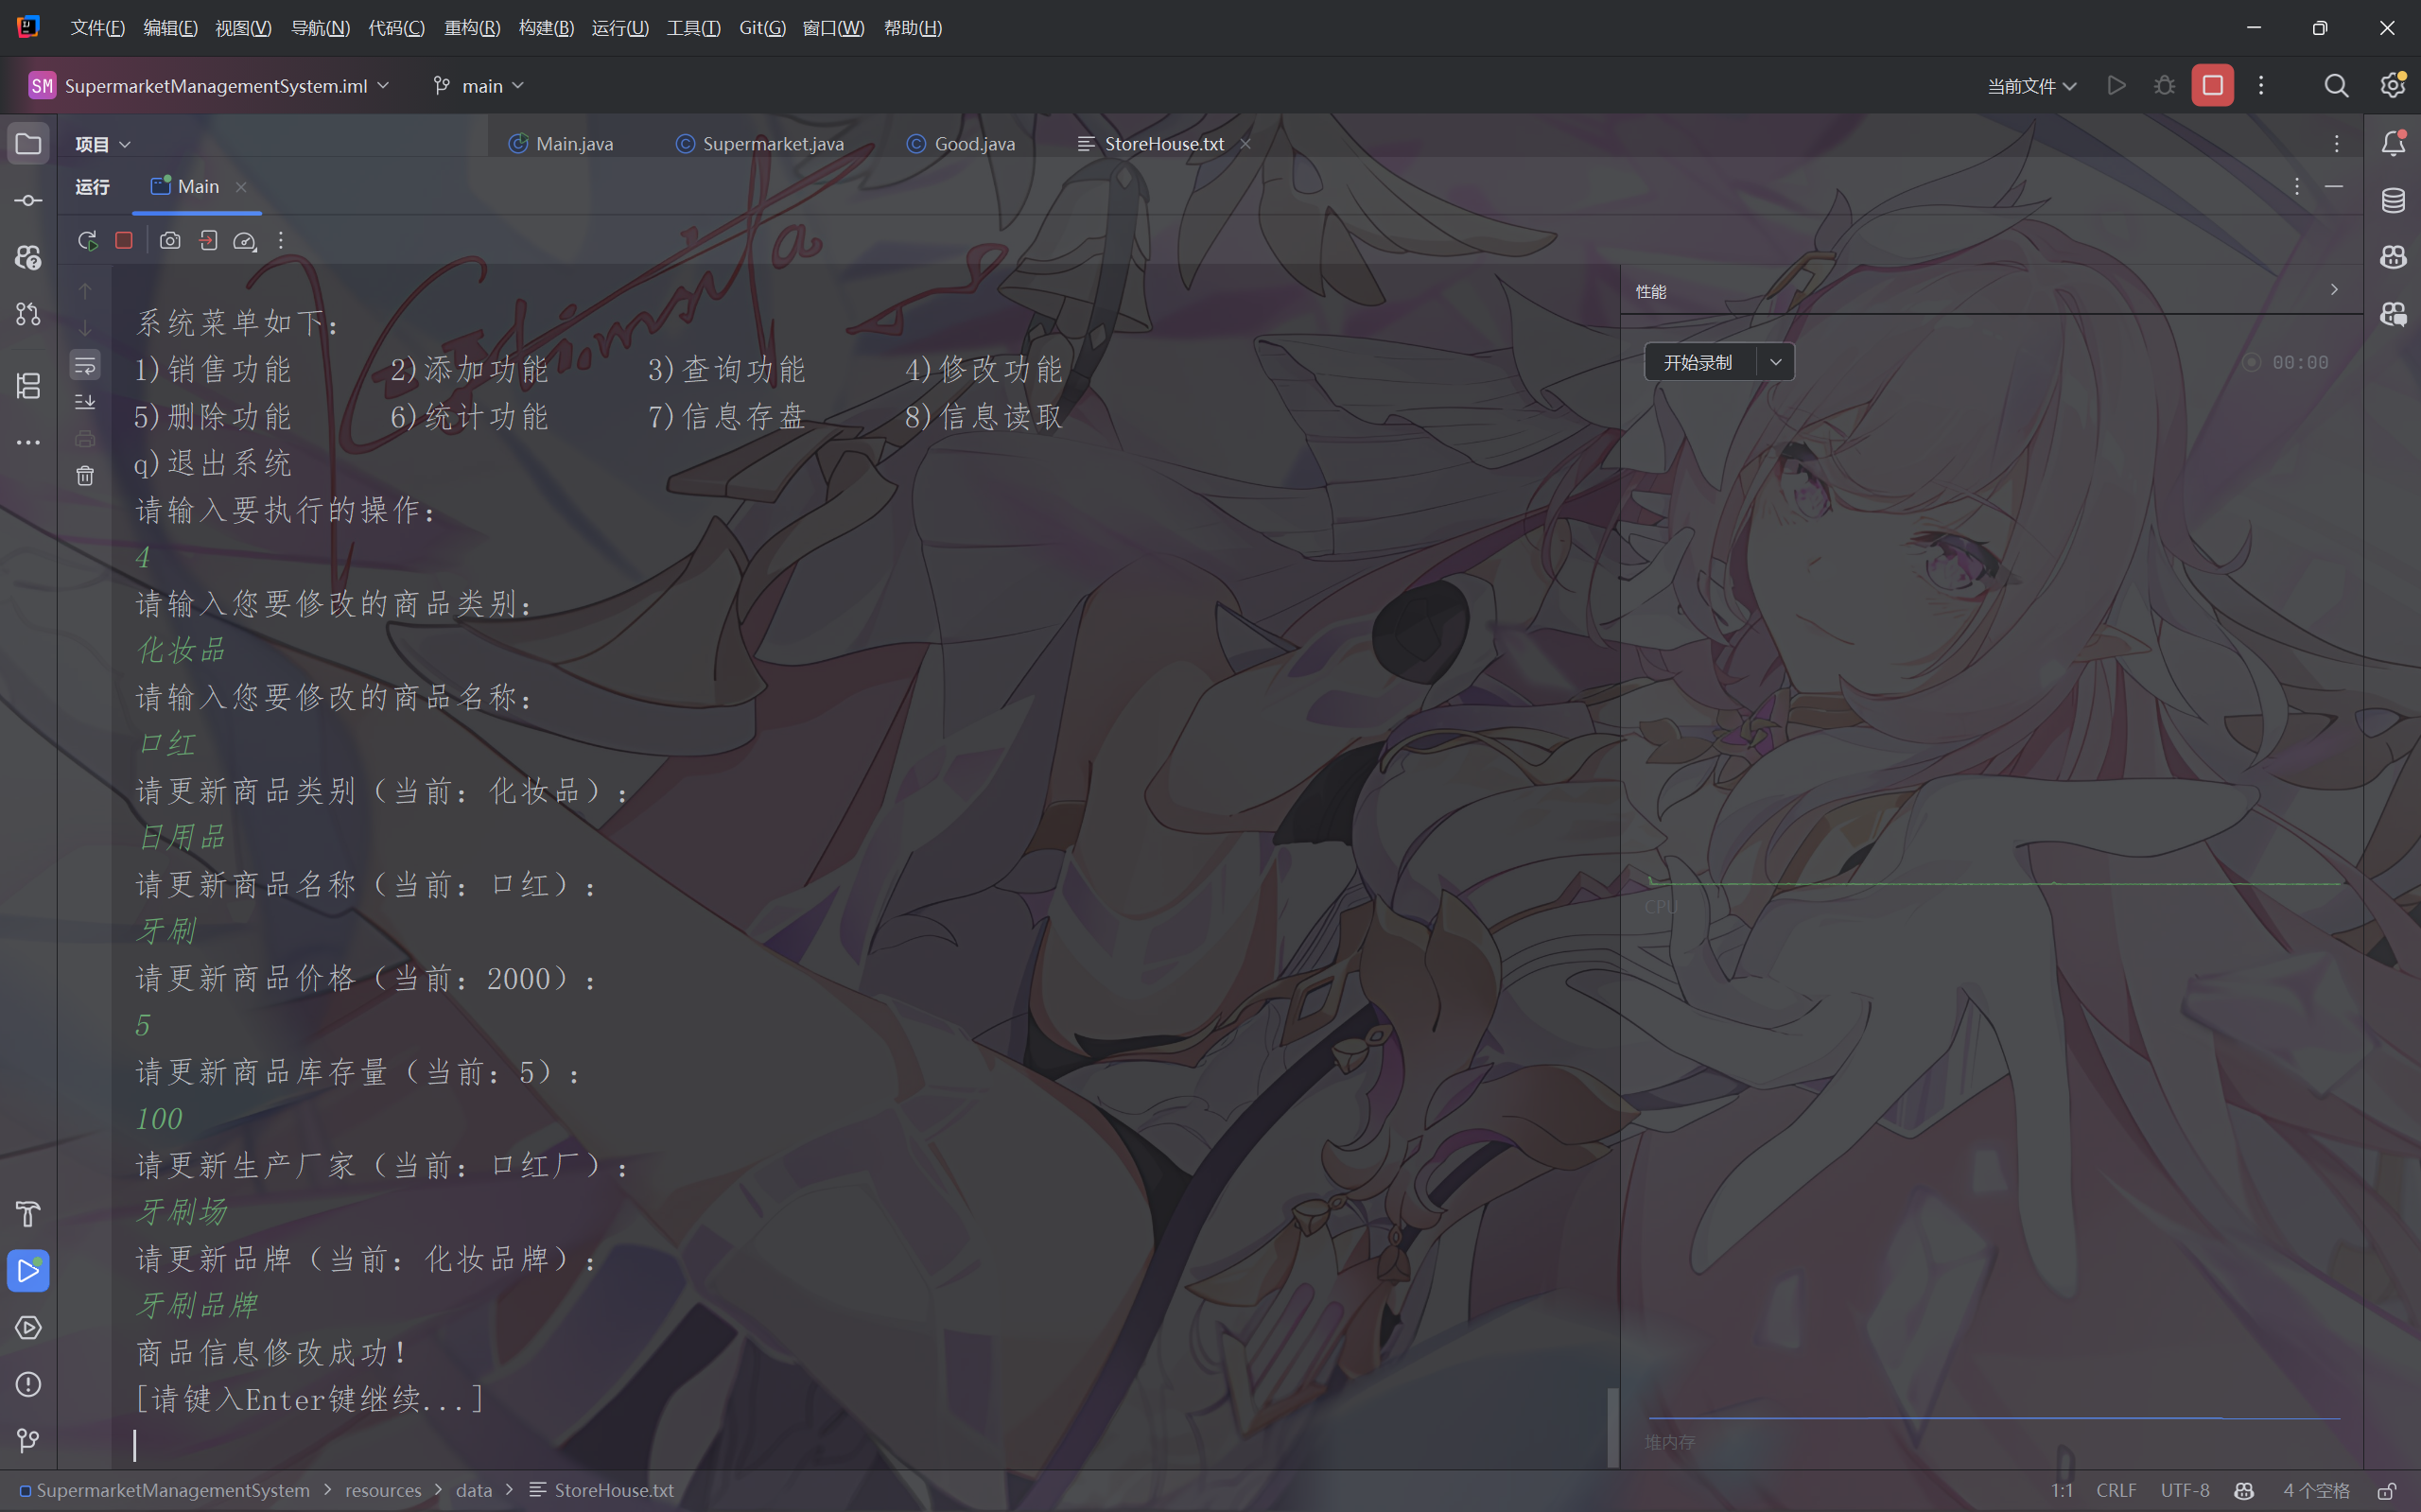
\includegraphics[width=\textwidth]{images/修改商品信息.png}
        \caption*{修改商品信息}
    \end{minipage}
    \hfill
    \begin{minipage}[t]{0.48\textwidth}
        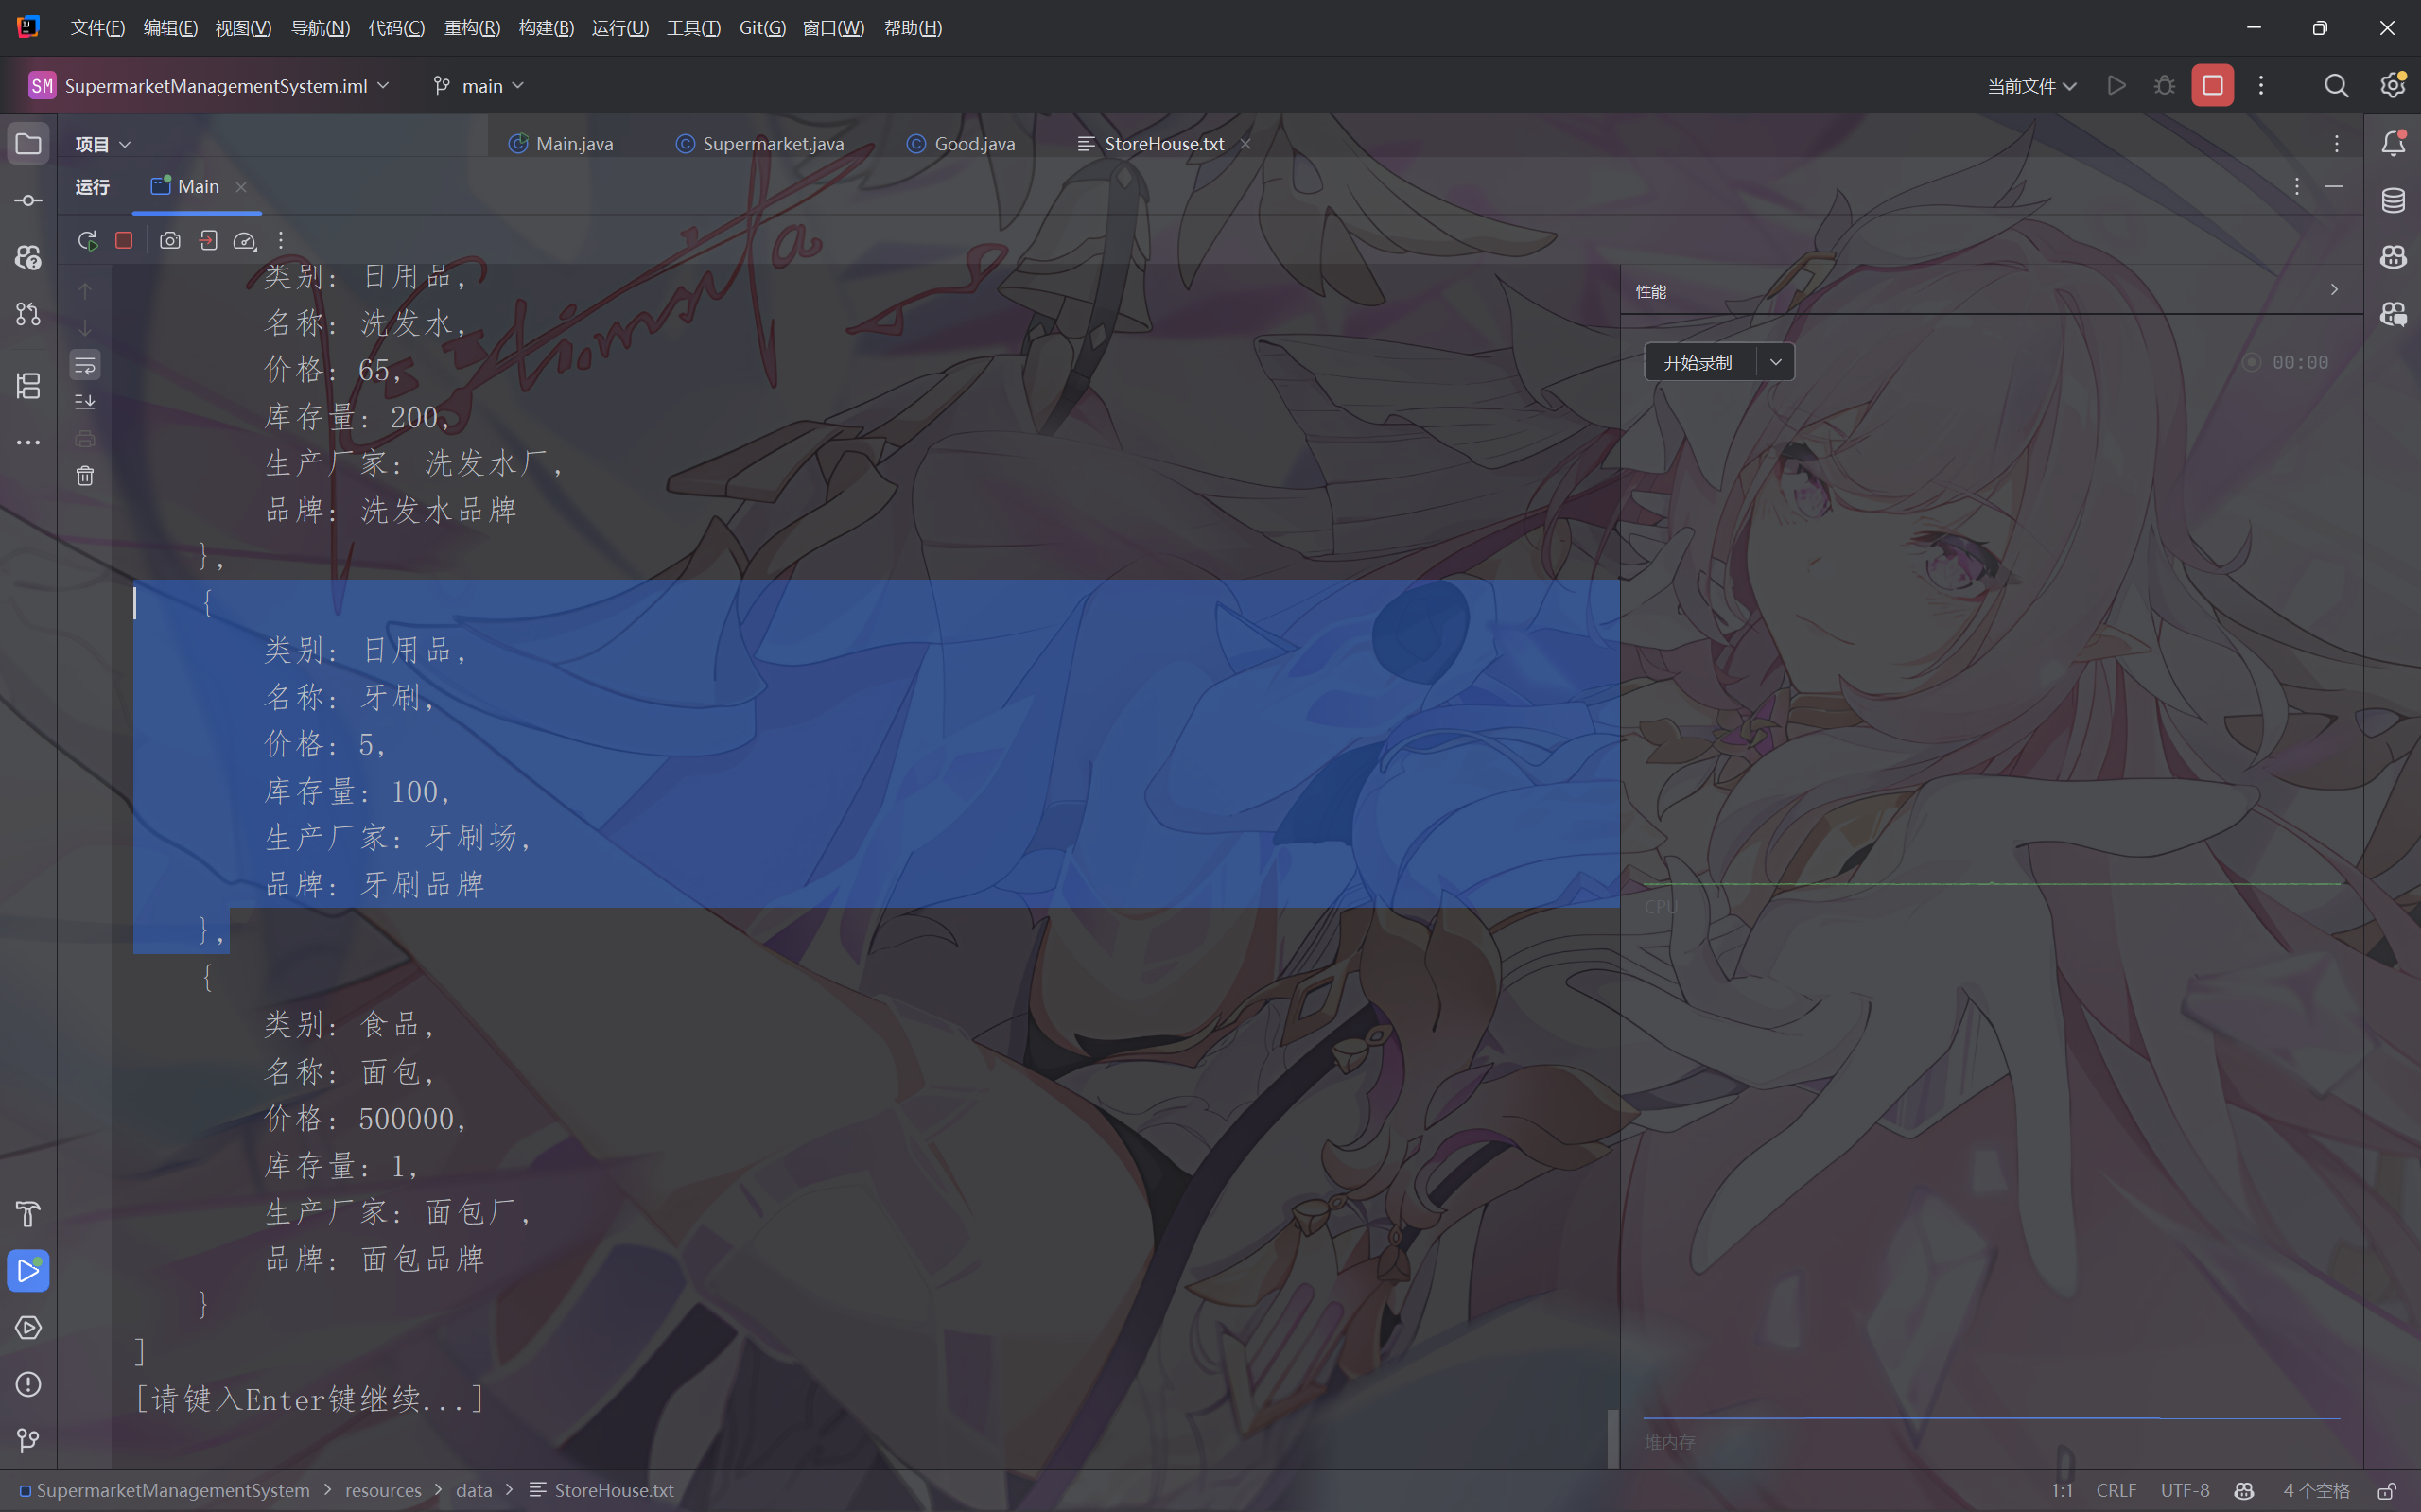
\includegraphics[width=\textwidth]{images/修改商品时库存信息随之改变.png}
        \caption*{修改商品时库存信息随之改变}
    \end{minipage}
\end{figure}

\begin{figure}[H]
    \begin{minipage}[t]{0.48\textwidth}
        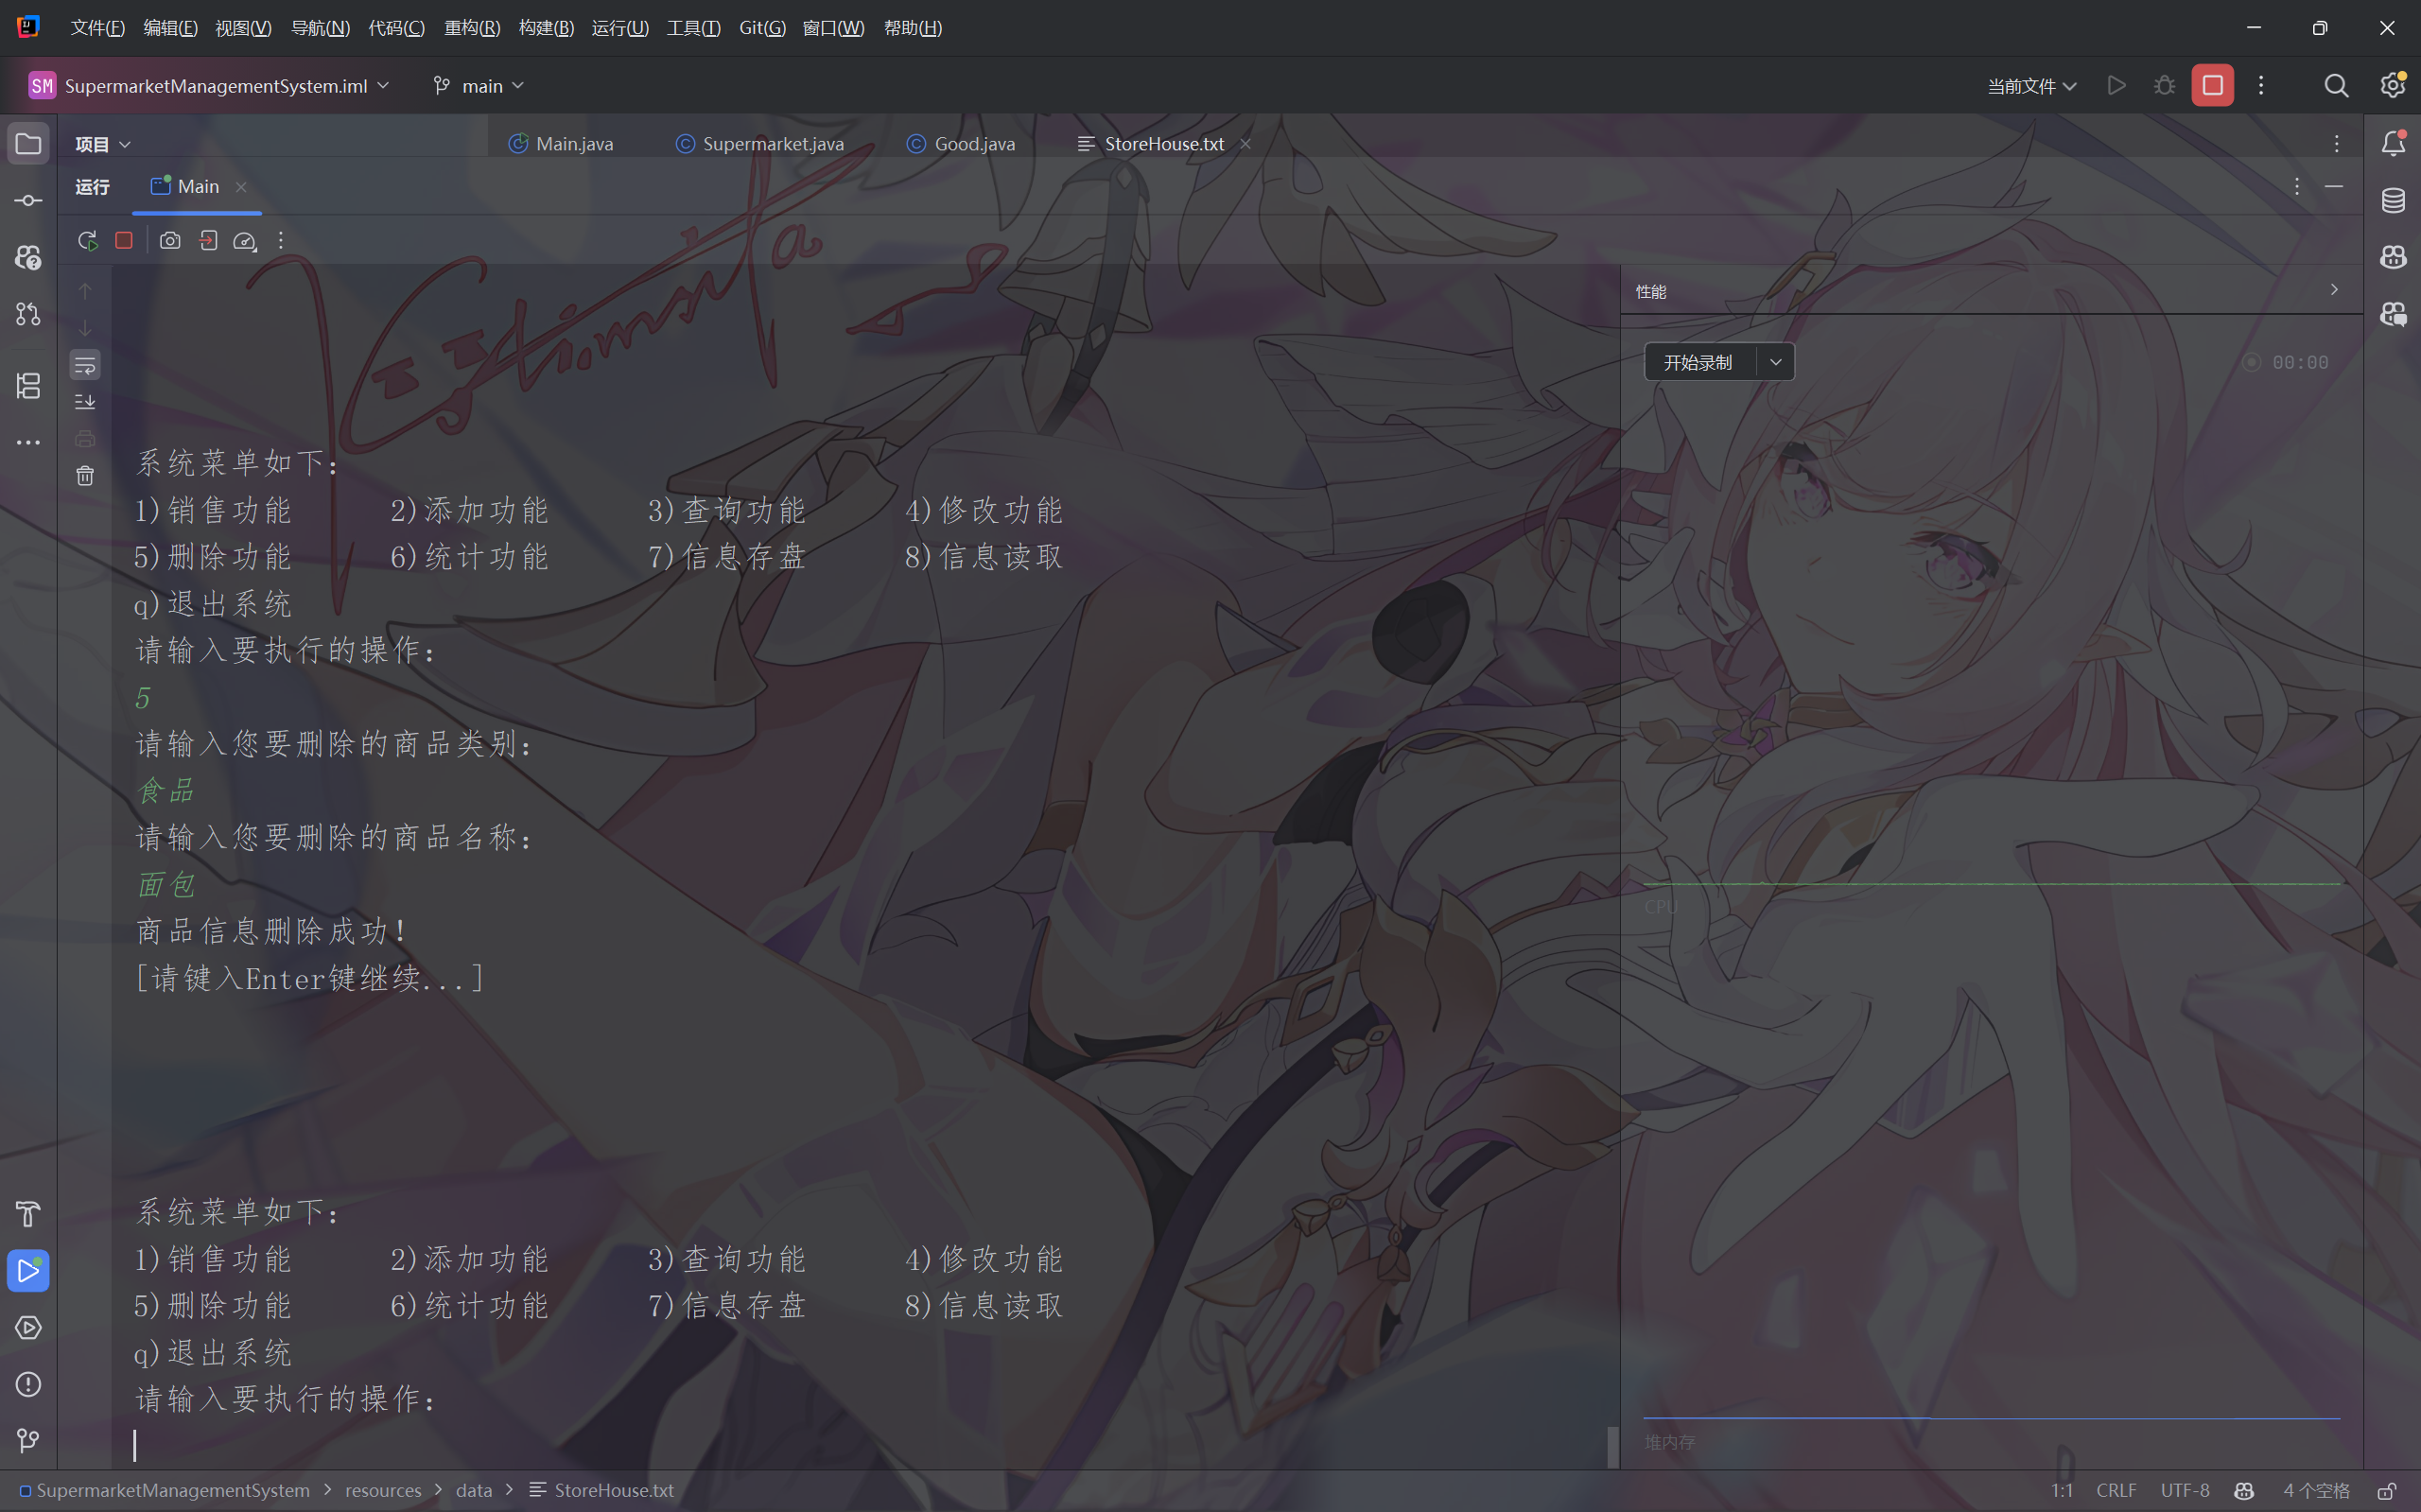
\includegraphics[width=\textwidth]{images/删除商品.png}
        \caption*{删除商品}
    \end{minipage}
    \hfill
    \begin{minipage}[t]{0.48\textwidth}
        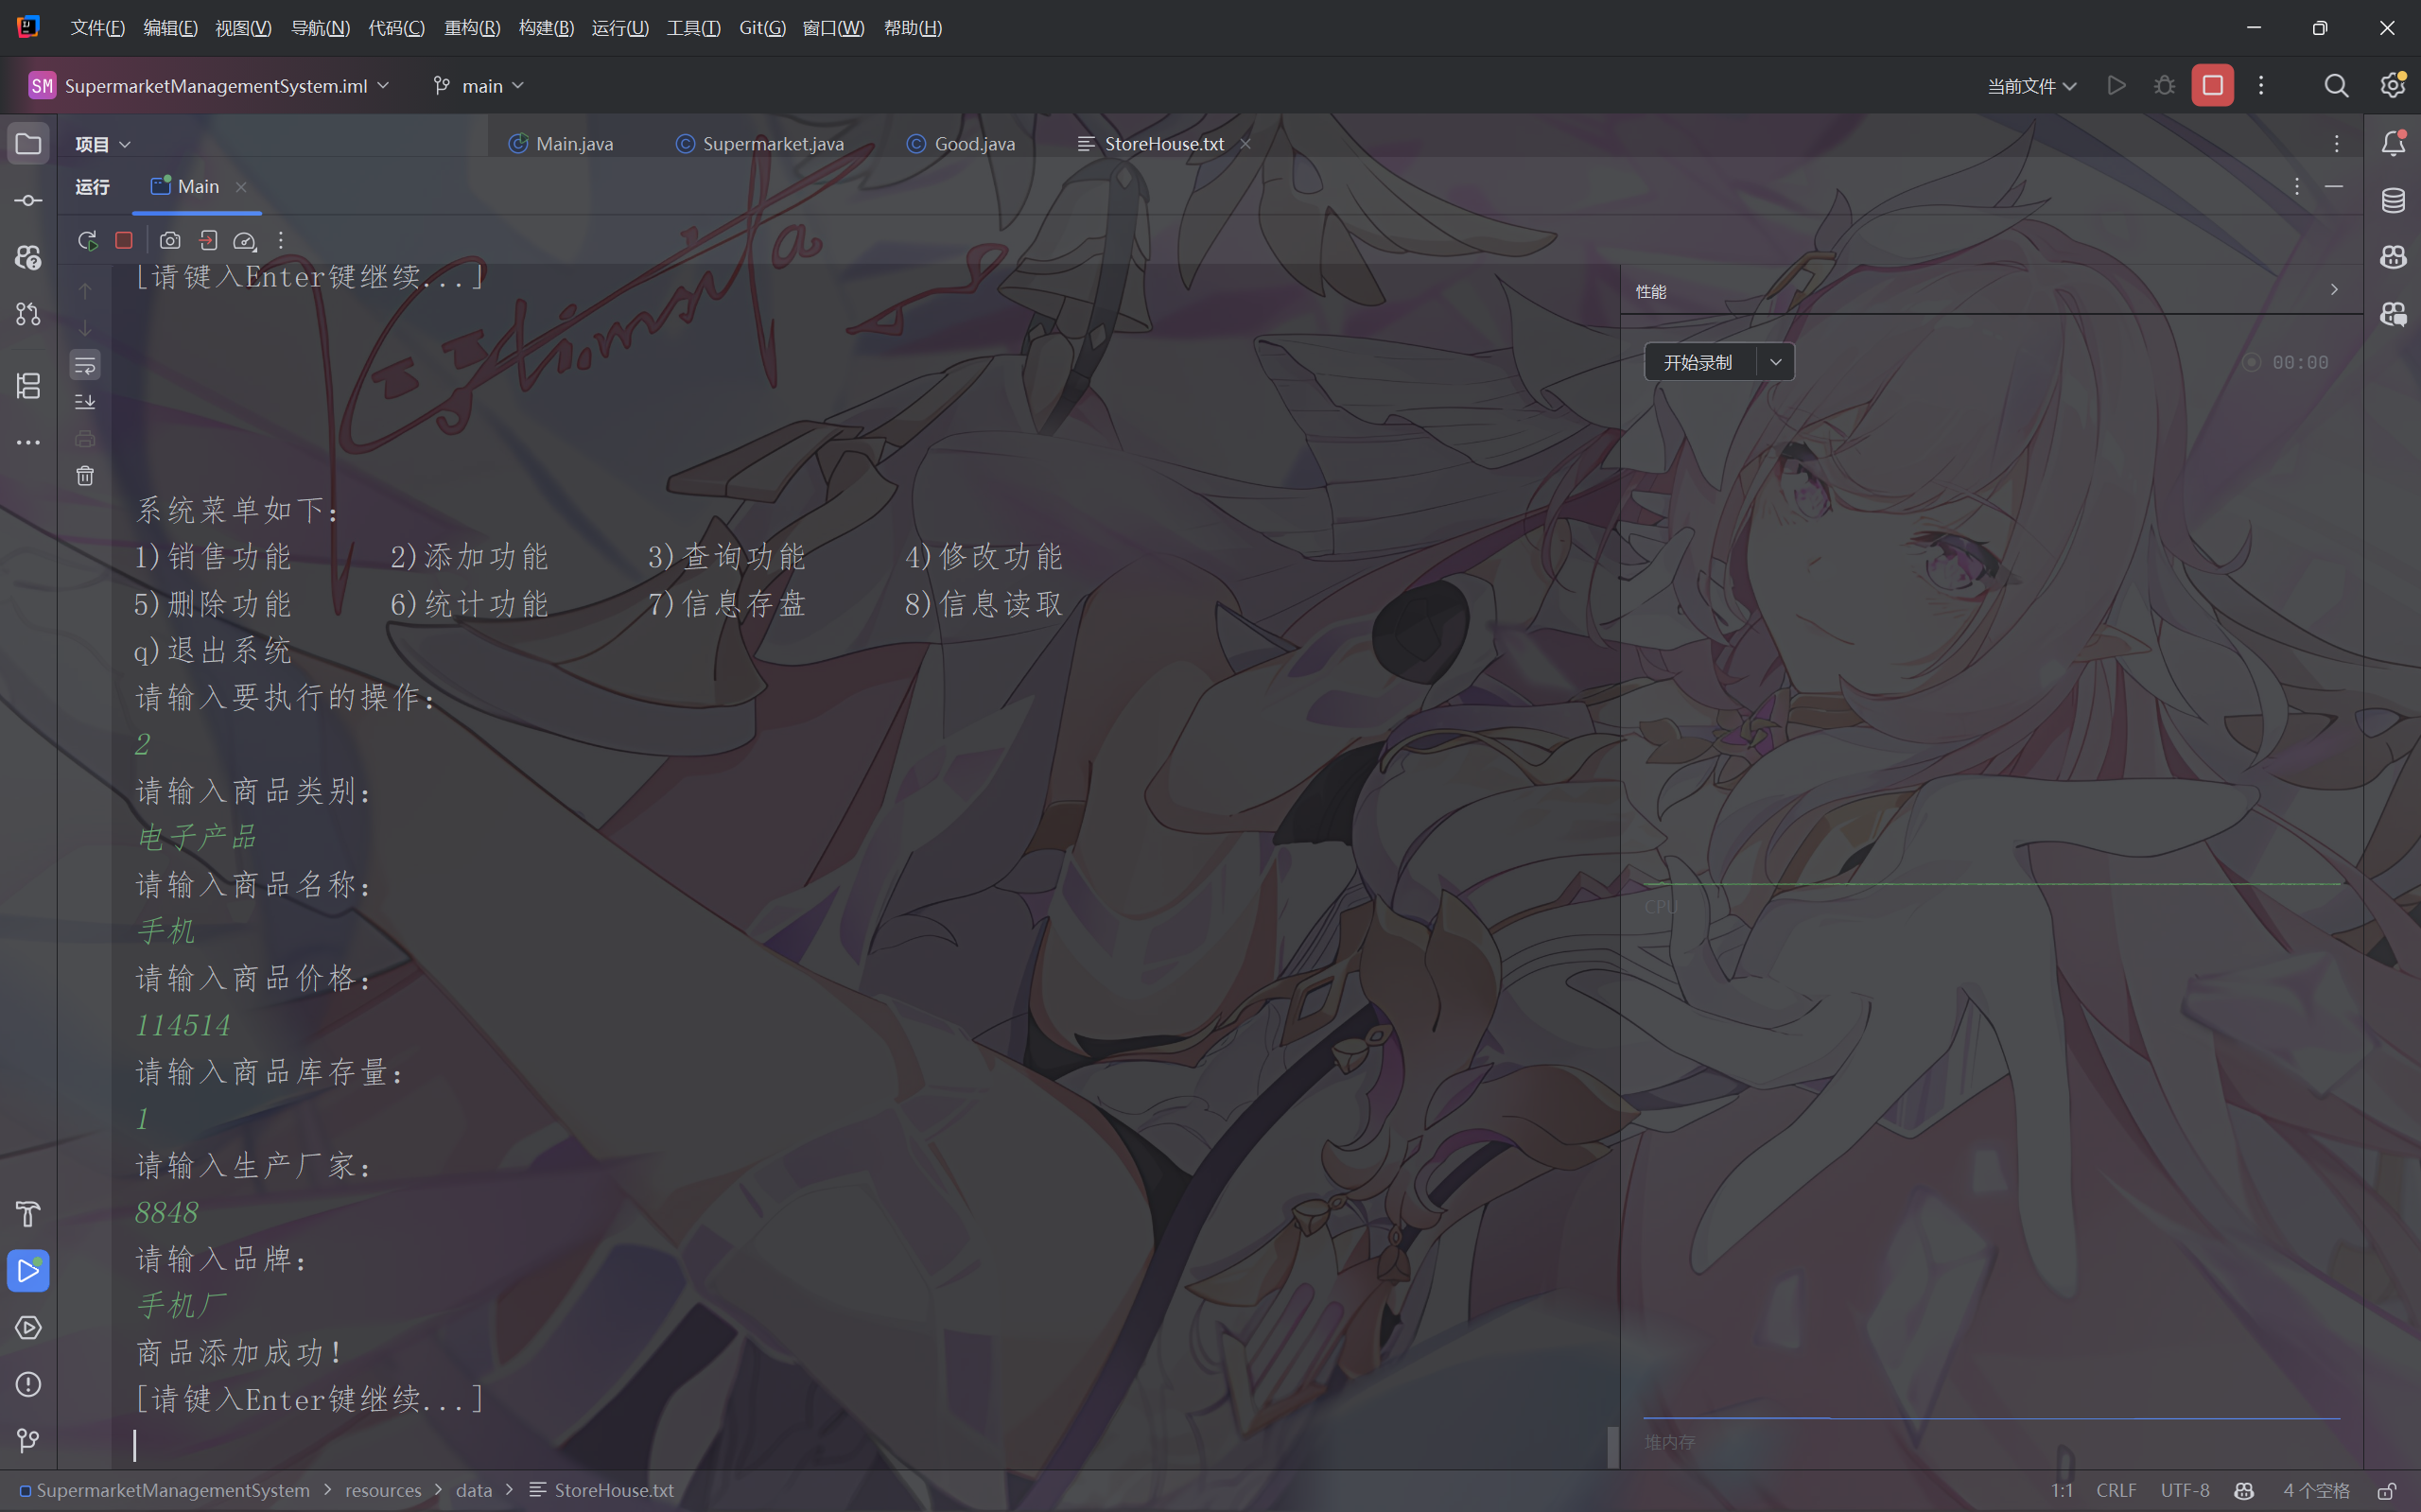
\includegraphics[width=\textwidth]{images/商品添加.png}
        \caption*{商品添加}
    \end{minipage}
\end{figure}

\begin{figure}[H]
    \begin{minipage}[t]{0.48\textwidth}
        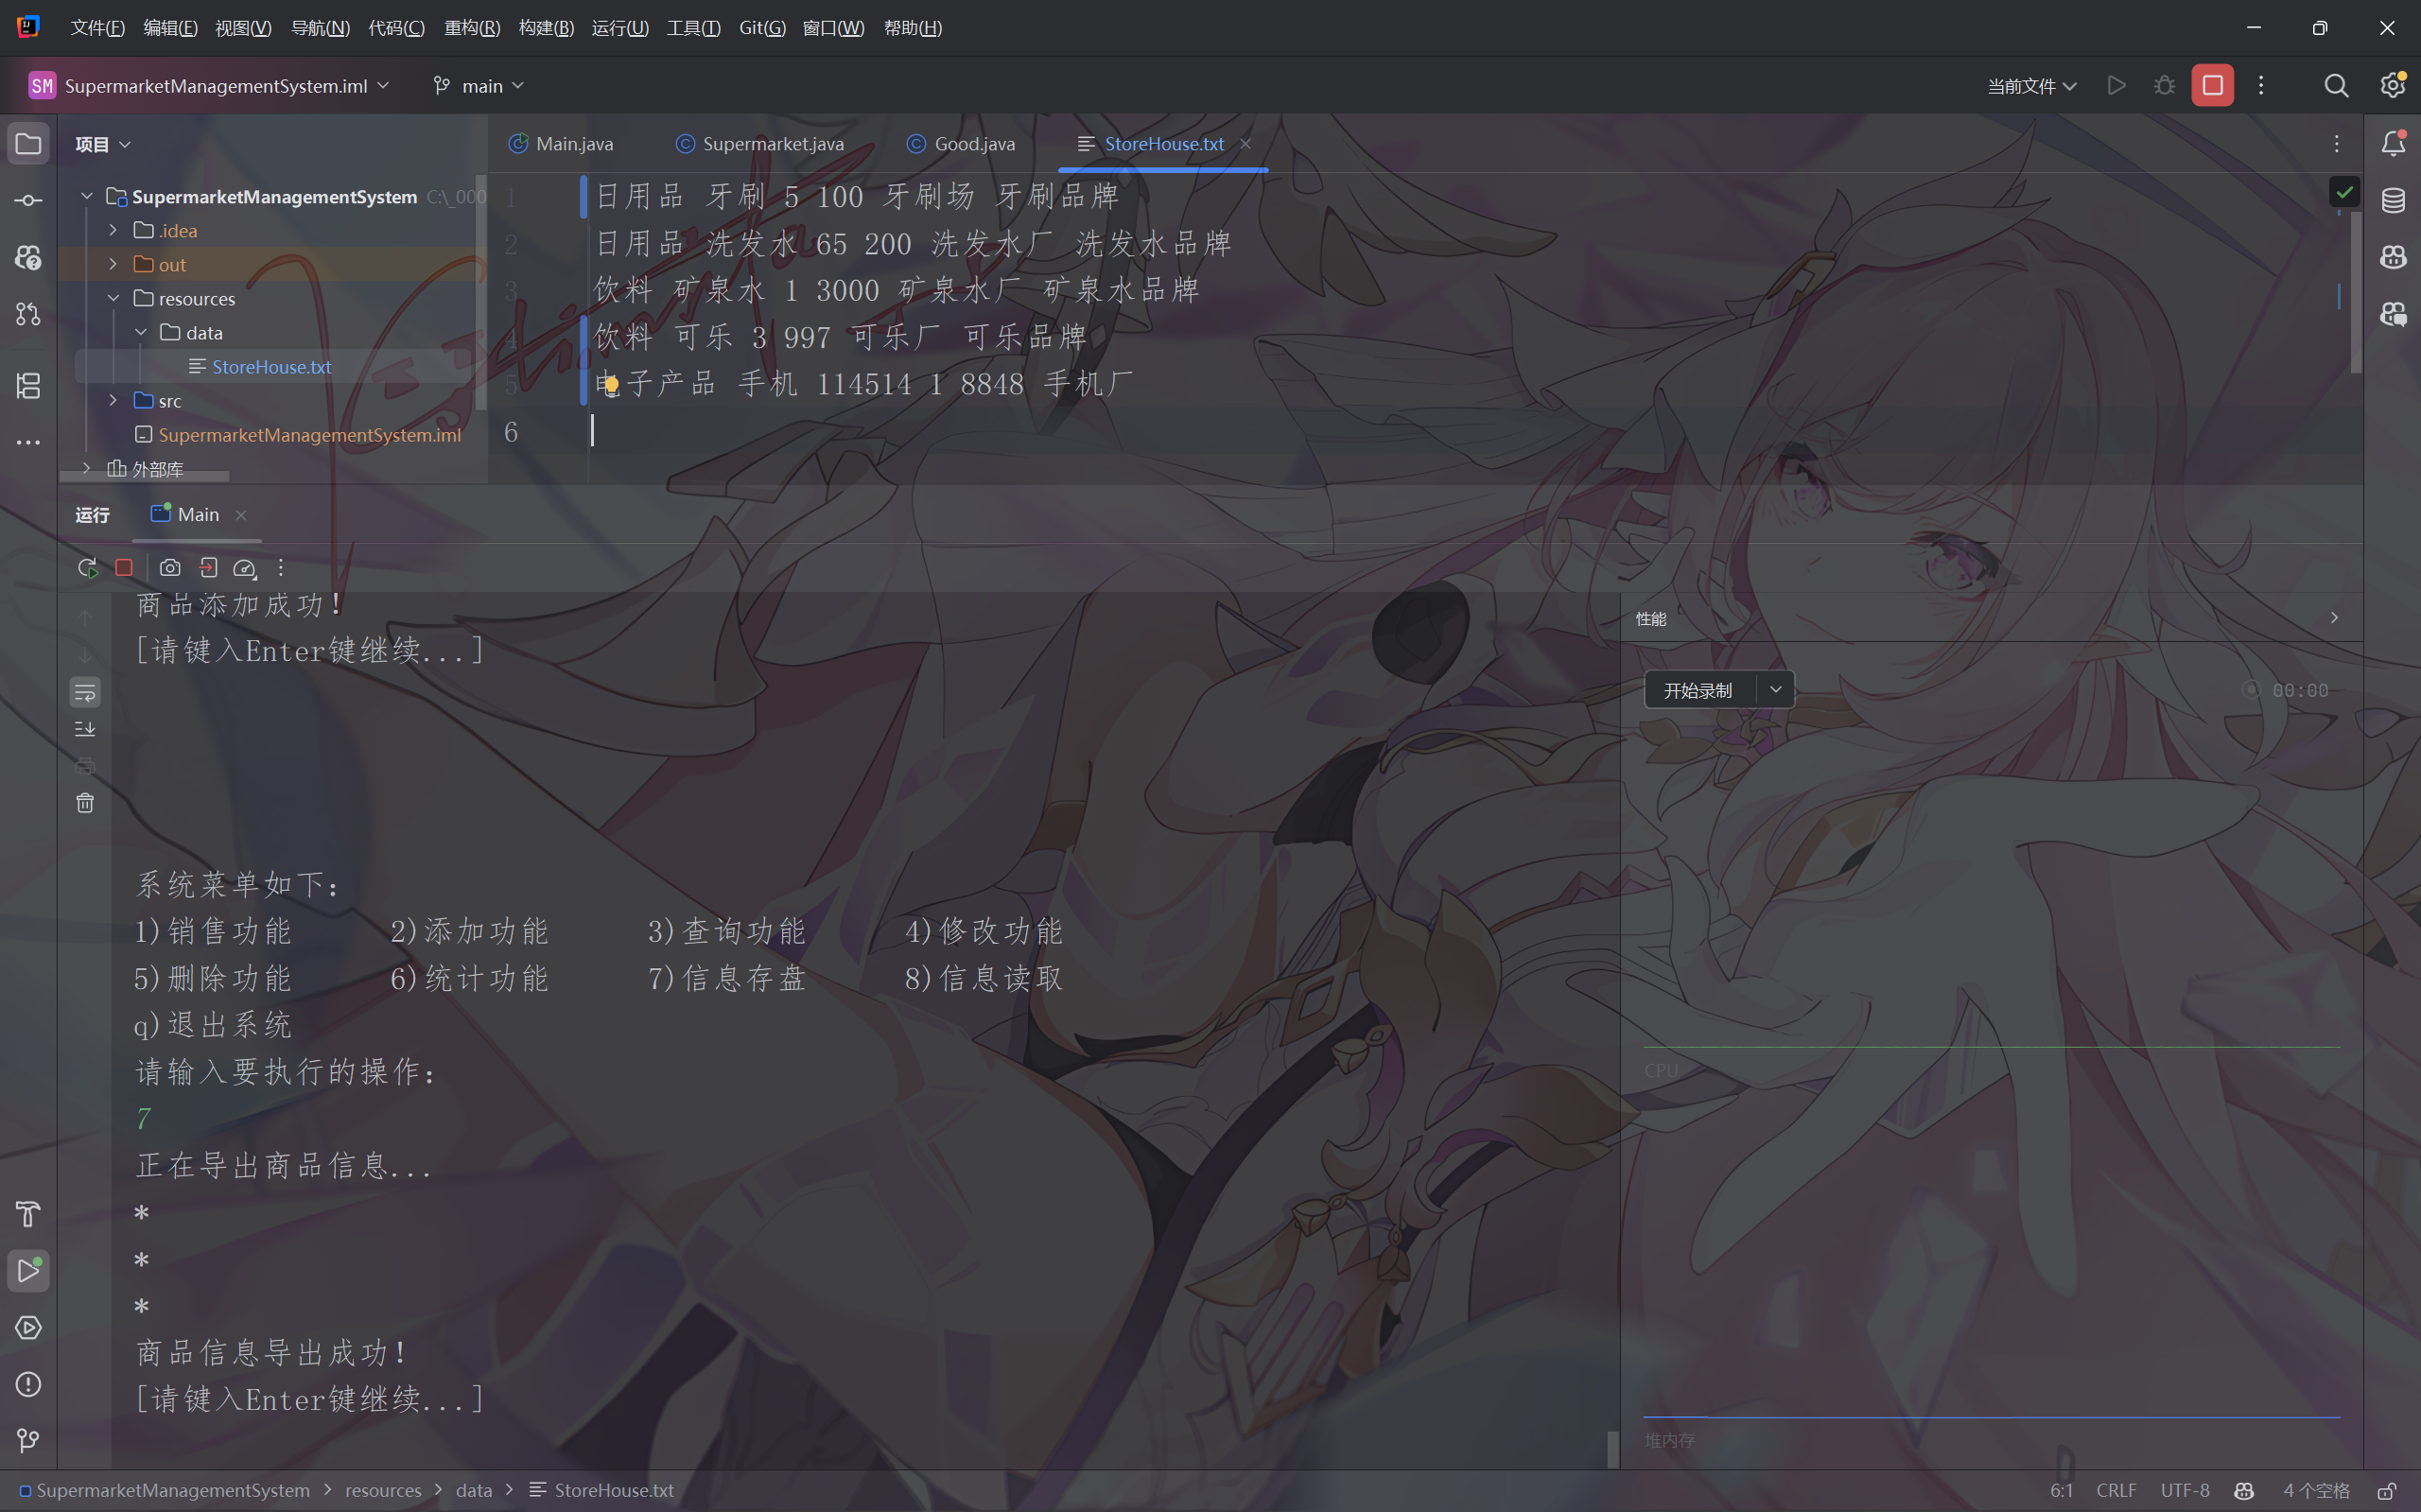
\includegraphics[width=\textwidth]{images/导出商品信息.png}
        \caption*{导出商品信息}
    \end{minipage}
    \hfill
    \begin{minipage}[t]{0.48\textwidth}
        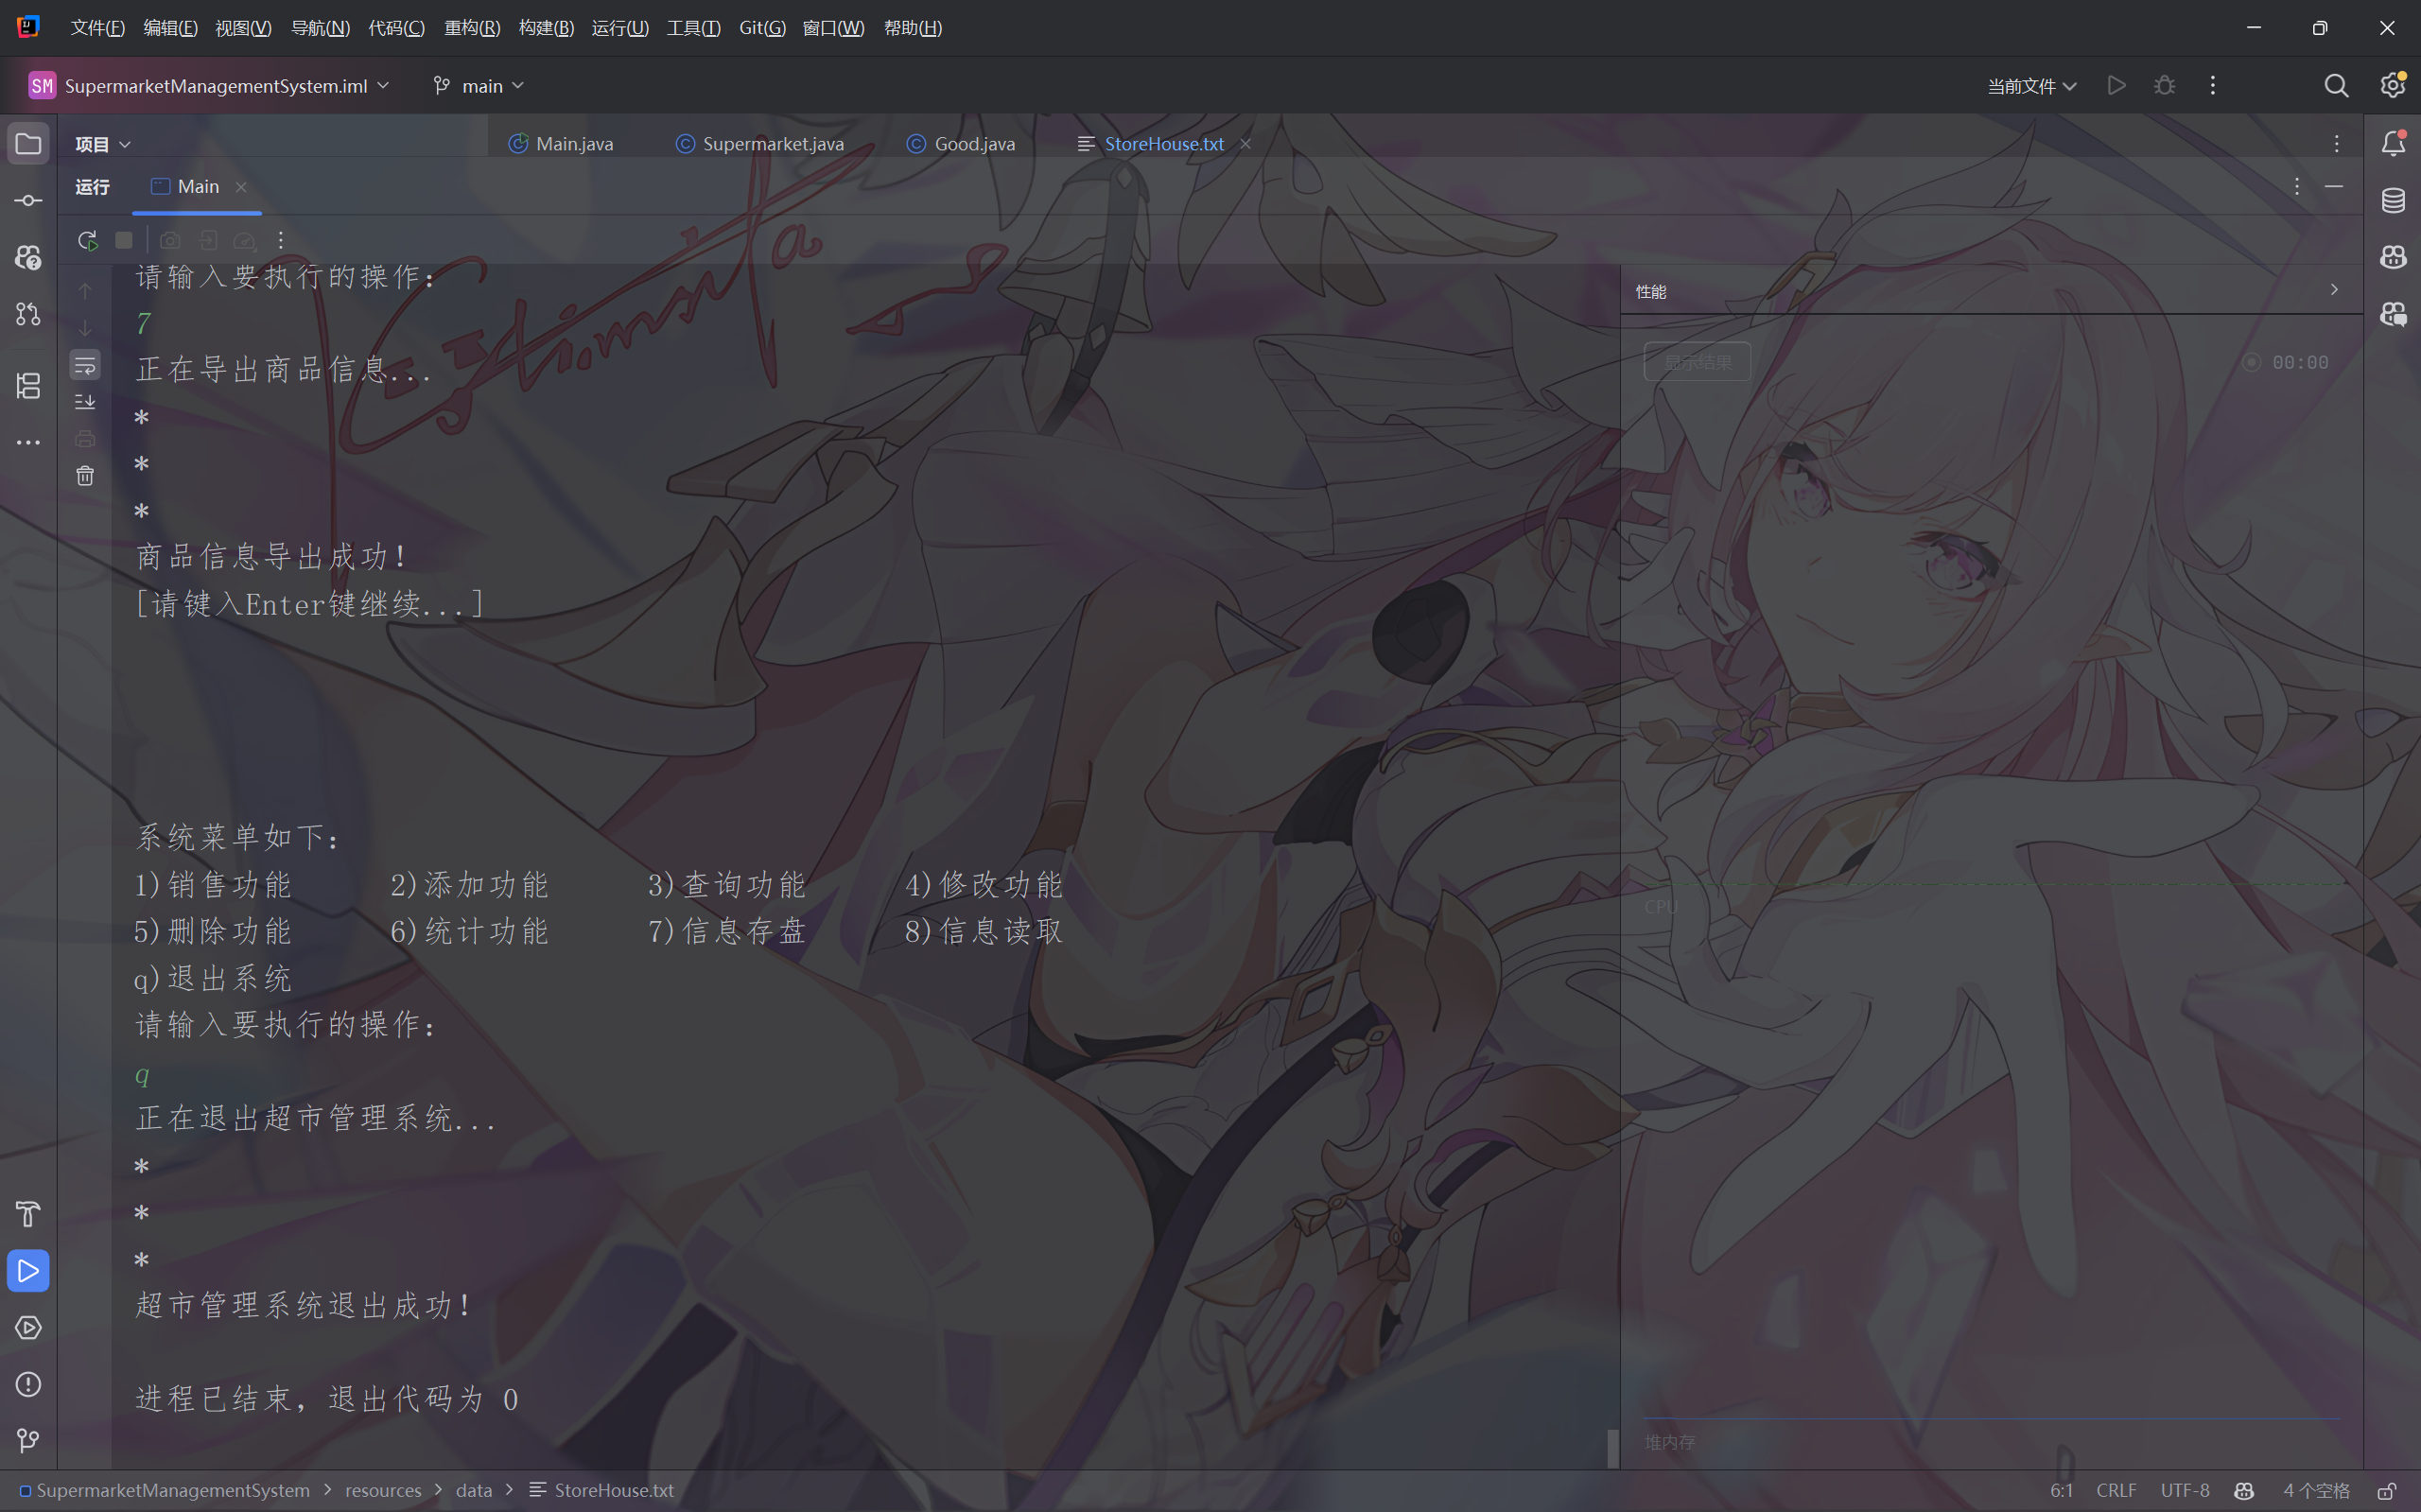
\includegraphics[width=\textwidth]{images/结束系统调用.png}
        \caption*{结束系统调用}
    \end{minipage}
\end{figure}

\section{总结}

\begin{flushleft}
本次实验项目基于 Java 语言开发,结合了面向对象编程思想和实际应用场景,实现了对商品仓库数据的管理。系统功能包括商品的添加、查询、修改、删除、销售和统计等,满足了超市商品管理的基本需求。
\end{flushleft}

\end{document}